\documentclass[10pt]{article}
\usepackage[utf8]{inputenc}
\usepackage[T1]{fontenc}
\usepackage{amsmath}
\usepackage{amsfonts}
\usepackage{amssymb}
\usepackage[version=4]{mhchem}
\usepackage{stmaryrd}
\usepackage{mathrsfs}
\usepackage{bbold}
\usepackage{graphicx}
\usepackage[export]{adjustbox}
\graphicspath{ {./images/} }
\usepackage{fvextra, csquotes}

\begin{document}
and $W$; and because it can also be thought of as $-\mathscr{L}_{g W}(f V)$, it satisfies a product rule in $f$ and $V$ as well. Expanding out these two product rules yields (8.11).

If $V$ and $W$ are vector fields on $M$ and $\theta$ is the flow of $V$, the Lie derivative $\left(\mathscr{L}_{V} W\right)_{p}$, by definition, expresses the $t$-derivative of the time-dependent vector $d\left(\theta_{-t}\right)_{\theta_{t}(p)}\left(W_{\theta_{t}(p)}\right) \in T_{p} M$ at $t=0$. The next proposition shows how it can also be used to compute the derivative of this expression at other times. We will use this result in the proof of Theorem 9.42 below.

Proposition 9.41. Suppose $M$ is a smooth manifold with or without boundary and $V, W \in \mathfrak{X}(M)$. If $\partial M \neq \varnothing$, assume also that $V$ is tangent to $\partial M$. Let $\theta$ be the flow of $V$. For any ( $t_{0}, p$ ) in the domain of $\theta$,

$$
\left.\frac{d}{d t}\right|_{t=t_{0}} d\left(\theta_{-t}\right)_{\theta_{t}(p)}\left(W_{\theta_{t}(p)}\right)=d\left(\theta_{-t_{0}}\right)\left(\left(\mathscr{L}_{V} W\right)_{\theta_{t_{0}}(p)}\right)
$$

Proof. Let $p \in M$ be arbitrary, let $\mathscr{D}^{(p)} \subseteq \mathbb{R}$ denote the domain of the integral curve $\theta^{(p)}$, and consider the map $X: \mathscr{D}^{(p)} \rightarrow T_{p} M$ given by $X(t)=$ $d\left(\theta_{-t}\right)_{\theta_{t}(p)}\left(W_{\theta_{t}(p)}\right)$. The argument in the proof of Lemma 9.36 shows that $X$ is a smooth curve in the vector space $T_{p} M$. Making the change of variables $t=t_{0}+s$, we obtain

$$
\begin{aligned}
X^{\prime}\left(t_{0}\right) & =\left.\frac{d}{d s}\right|_{s=0} X\left(t_{0}+s\right)=\left.\frac{d}{d s}\right|_{s=0} d\left(\theta_{-t_{0}-s}\right)\left(W_{\theta_{s+t_{0}}}(p)\right) \\
& =\left.\frac{d}{d s}\right|_{s=0} d\left(\theta_{-t_{0}}\right) \circ d\left(\theta_{-s}\right)\left(W_{\theta_{s}\left(\theta_{t_{0}}(p)\right.}\right) \\
& =d\left(\theta_{-t_{0}}\right)\left(\left.\frac{d}{d s}\right|_{s=0} d\left(\theta_{-s}\right)\left(W_{\theta_{s}\left(\theta_{t_{0}}(p)\right)}\right)\right)
\end{aligned}
$$

(The last equality follows because $d\left(\theta_{-t_{0}}\right): T_{\theta_{t_{0}}(p)} M \rightarrow T_{p} M$ is a linear map that is independent of $s$. See Fig. 9.14.) By definition of the Lie derivative, this last expression is equal to the right-hand side of (9.17).

\section*{Commuting Vector Fields}
Let $M$ be a smooth manifold and $V, W \in \mathfrak{X}(M)$. We say that $\boldsymbol{V}$ and $\boldsymbol{W}$ commute if $V W f=W V f$ for every smooth function $f$, or equivalently if $[V, W] \equiv 0$. If $\theta$ is a smooth flow, a vector field $W$ is said to be invariant under $\boldsymbol{\theta}$ if $W$ is $\theta_{t}$-related to itself for each $t$; more precisely, this means that $\left.W\right|_{M_{t}}$ is $\theta_{t}$-related to $\left.W\right|_{M_{-t}}$ for each $t$, or equivalently that $d\left(\theta_{t}\right)_{p}\left(W_{p}\right)=W_{\theta_{t}(p)}$ for all $(t, p)$ in the domain of $\theta$. The next proposition shows that these two concepts are intimately related.

Theorem 9.42. For smooth vector fields $V$ and $W$ on a smooth manifold $M$, the following are equivalent:\\
(a) $V$ and $W$ commute.\\
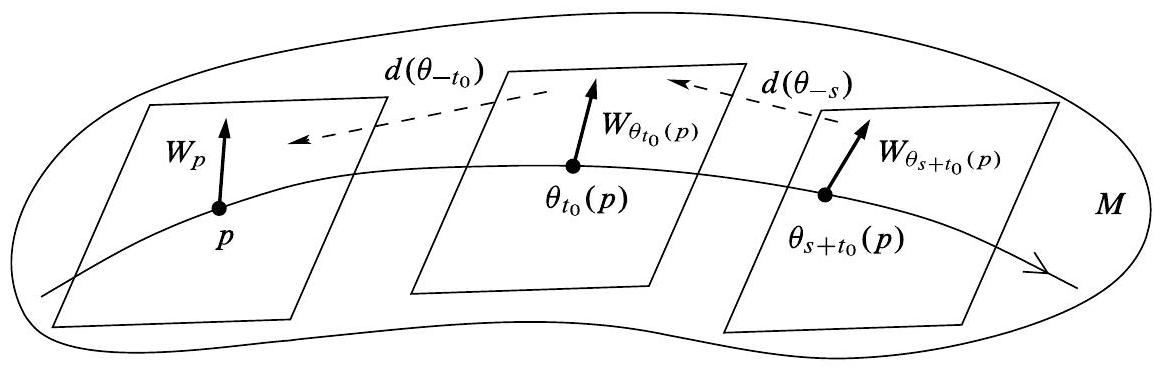
\includegraphics[max width=\textwidth, center]{2025_06_03_90f64b1a1e243cccc2e0g-250}

Fig. 9.14 Proof of Proposition 9.41\\
(b) $W$ is invariant under the flow of $V$.\\
(c) $V$ is invariant under the flow of $W$.

Proof. Suppose $V, W \in \mathfrak{X}(M)$, and let $\theta$ denote the flow of $V$. If (b) holds, then $W_{\theta_{t}(p)}=d\left(\theta_{t}\right)_{p}\left(W_{p}\right)$ whenever $(t, p)$ is in the domain of $\theta$. Applying $d\left(\theta_{-t}\right)_{\theta_{t}(p)}$ to both sides, we conclude that $d\left(\theta_{-t}\right)_{\theta_{t}(p)}\left(W_{\theta_{t}(p)}\right)=W_{p}$, which obviously implies $[V, W]=\mathscr{L}_{V} W=0$ directly from the definition of the Lie derivative. The same argument shows that (c) implies (a).

To prove that (a) implies (b), assume that $[V, W]=\mathscr{L}_{V} W=0$. Let $p \in M$ be arbitrary, and let $X(t)=d\left(\theta_{-t}\right)_{\theta_{t}(p)}\left(W_{\theta_{t}(p)}\right)$ for $t \in \mathscr{D}^{(p)}$. Proposition 9.41 shows that $X^{\prime}(t) \equiv 0$. Since $X(0)=W_{p}$, this implies that $X(t)=W_{p}$ for all $t \in \mathscr{D}^{(p)}$, and applying $d\left(\theta_{t}\right)_{p}$ to both sides yields the identity that says $W$ is invariant under $\theta$. The same proof also shows that (a) implies (c).

Corollary 9.43. Every smooth vector field is invariant under its own flow.\\
Proof. Use the preceding proposition together with the fact that $[V, V] \equiv 0$.\\
The deepest characterization of commuting vector fields is in terms of the relationship between their respective flows. The next theorem says that two vector fields commute if and only if their flows commute. But before we state the theorem formally, we need to examine exactly what this means. Suppose $V$ and $W$ are smooth vector fields on $M$, and let $\theta$ and $\psi$ denote their respective flows. If $V$ and $W$ are complete, it is clear what we should mean by saying their flows commute: simply that $\theta_{t} \circ \psi_{s}=\psi_{s} \circ \theta_{t}$ for all $s, t \in \mathbb{R}$. However, if either $V$ or $W$ is not complete, the most we can hope for is that this equation holds for all $s$ and $t$ such that both sides are defined. Unfortunately, even when the vector fields commute, their flows might not commute in this naive sense, because there are examples of commuting vector fields $V$ and $W$ and particular choices of $t, s$, and $p$ for which both $\theta_{t} \circ \psi_{s}(p)$ and $\psi_{s} \circ \theta_{t}(p)$ are defined, but they are not equal (see Problem 9-19 for one such example). Here is the problem: if $\theta_{t} \circ \psi_{s}(p)$ is defined for $t=t_{0}$ and $s=s_{0}$, then by the properties of flow domains, it must be defined for all $t$ in some open interval containing 0 and $t_{0}$, but the analogous statement need not be true of $s$-there might be values of $s$ between 0 and $s_{0}$ for which the integral curve of $V$ starting at $\psi_{s}(p)$ does not extend all the way to $t=t_{0}$.

Thus we make the following definition. If $\theta$ and $\psi$ are flows on $M$, we say that $\boldsymbol{\theta}$ and $\boldsymbol{\psi}$ commute if the following condition holds for every $p \in M$ : whenever $J$ and $K$ are open intervals containing 0 such that one of the expressions $\theta_{t} \circ \psi_{s}(p)$ or $\psi_{s} \circ \theta_{t}(p)$ is defined for all $(s, t) \in J \times K$, both are defined and they are equal. For global flows, this is the same as saying that $\theta_{t} \circ \psi_{s}=\psi_{s} \circ \theta_{t}$ for all $s$ and $t$.\\
Theorem 9.44. Smooth vector fields commute if and only if their flows commute.\\
Proof. Let $V$ and $W$ be smooth vector fields on a smooth manifold $M$, and let $\theta$ and $\psi$ denote their respective flows. Assume first that $V$ and $W$ commute. Suppose that $p \in M$, and $J$ and $K$ are open intervals containing 0 such that $\psi_{s} \circ \theta_{t}(p)$ is defined for all $(s, t) \in J \times K$. (The same proof with $V$ and $W$ reversed works under the assumption that the other expression is defined on such a rectangle.) By Theorem 9.42, the hypothesis implies that $V$ is invariant under $\psi$. Fix any $s \in J$, and consider the curve $\gamma: K \rightarrow M$ defined by $\gamma(t)=\psi_{s} \circ \theta_{t}(p)=\psi_{s}\left(\theta^{(p)}(t)\right)$. This curve satisfies $\gamma(0)=\psi_{s}(p)$, and its velocity at $t \in K$ is

$$
\gamma^{\prime}(t)=\frac{d}{d t}\left(\psi_{s}\left(\theta^{(p)}(t)\right)\right)=d\left(\psi_{s}\right)\left(\theta^{(p)^{\prime}}(t)\right)=d\left(\psi_{s}\right)\left(V_{\theta^{(p)}(t)}\right)=V_{\gamma(t)}
$$

Thus, $\gamma$ is an integral curve of $V$ starting at $\psi_{s}(p)$. By uniqueness, therefore,

$$
\gamma(t)=\theta^{\psi_{s}(p)}(t)=\theta_{t}\left(\psi_{s}(p)\right) .
$$

This proves that $\theta$ and $\psi$ commute.\\
Conversely, assume that the flows commute, and let $p \in M$. If $\varepsilon>0$ is chosen small enough that $\psi_{s} \circ \theta_{t}(p)$ is defined whenever $|s|<\varepsilon$ and $|t|<\varepsilon$, then the hypothesis guarantees that $\psi_{s} \circ \theta_{t}(p)=\theta_{t} \circ \psi_{s}(p)$ for all such $s$ and $t$. This can be rewritten in the form

$$
\psi^{\theta_{t}(p)}(s)=\theta_{t}\left(\psi^{(p)}(s)\right)
$$

Differentiating this relation with respect to $s$, we get

$$
W_{\theta_{t}(p)}=\left.\frac{d}{d s}\right|_{s=0} \psi^{\theta_{t}(p)}(s)=\left.\frac{d}{d s}\right|_{s=0} \theta_{t}\left(\psi^{(p)}(s)\right)=d\left(\theta_{t}\right)_{p}\left(W_{p}\right)
$$

Applying $d\left(\theta_{-t}\right)_{\theta_{t}(p)}$ to both sides, we conclude

$$
d\left(\theta_{-t}\right)_{\theta_{t}(p)}\left(W_{\theta_{t}(p)}\right)=W_{p}
$$

Differentiating with respect to $t$ and applying the definition of the Lie derivative shows that $\left(\mathscr{L}_{V} W\right)_{p}=0$.

\section*{Commuting Frames}
Suppose $M$ is a smooth $n$-manifold. Recall that a local frame for $M$ is an $n$-tuple ( $E_{i}$ ) of vector fields defined on an open subset $U \subseteq M$ such that ( $\left.E_{i}\right|_{p}$ ) forms a basis for $T_{p} M$ at each $p \in U$. A smooth local frame ( $E_{i}$ ) for $M$ is called a commuting frame if $\left[E_{i}, E_{j}\right]=0$ for all $i$ and $j$. (Commuting frames are called holonomic frames by some authors.)

\section*{Example 9.45 (Commuting and Noncommuting Frames).}
(a) The simplest examples of commuting frames are the coordinate frames. Given any smooth coordinate chart $\left(U,\left(x^{i}\right)\right)$ for a smooth manifold $M$, (8.10) shows that the coordinate frame $\left(\partial / \partial x^{i}\right)$ is a commuting frame.\\
(b) The frame ( $E_{1}, E_{2}$ ) for $\mathbb{R}^{2}$ over $\mathbb{R}^{2} \backslash\{0\}$ defined by (8.3) is not a commuting frame, because a straightforward computation shows that

$$
\left[E_{1}, E_{2}\right]=\frac{y}{r^{2}} \frac{\partial}{\partial x}-\frac{x}{r^{2}} \frac{\partial}{\partial y} \neq 0 .
$$

Because every coordinate frame is a commuting frame, and because Lie brackets are invariantly defined, it follows that a necessary condition for a smooth frame to be expressible as a coordinate frame in some smooth chart is that it be a commuting frame. Thus, the computation above shows that ( $E_{1}, E_{2}$ ) cannot be expressed as a coordinate frame for $\mathbb{R}^{2}$ with respect to any choice of smooth local coordinates.

The next theorem shows that commuting is also a sufficient condition for a smooth frame to be locally expressible as a coordinate frame.

Theorem 9.46 (Canonical Form for Commuting Vector Fields). Let $M$ be a smooth $n$-manifold, and let $\left(V_{1}, \ldots, V_{k}\right)$ be a linearly independent $k$-tuple of smooth commuting vector fields on an open subset $W \subseteq M$. For each $p \in W$, there exists a smooth coordinate chart $\left(U,\left(s^{i}\right)\right)$ centered at $p$ such that $V_{i}=\partial / \partial s^{i}$ for $i=1, \ldots, k$. If $S \subseteq W$ is an embedded codimension- $k$ submanifold and $p$ is a point of $S$ such that $T_{p} S$ is complementary to the span of $\left(\left.V_{1}\right|_{p}, \ldots,\left.V_{k}\right|_{p}\right)$, then the coordinates can also be chosen such that $S \cap U$ is the slice defined by $s^{1}=\cdots=s^{k}=0$.

Proof. Let $p \in W$ be arbitrary. If no submanifold $S$ is given, just let $S$ be any smooth embedded codimension- $k$ submanifold $S$ whose tangent space at $p$ is complementary to the span of $\left(\left.V_{1}\right|_{p}, \ldots,\left.V_{k}\right|_{p}\right)$ (e.g., an appropriate coordinate slice). Let $\left(U,\left(x^{i}\right)\right)$ be a slice chart for $S$ centered at $p$, with $U \subseteq W$, and with $S \cap U$ equal to the slice $\left\{x \in U: x^{1}=\cdots=x^{k}=0\right\}$. Our assumptions ensure that the vectors $\left\{\left.V_{1}\right|_{p}, \ldots,\left.V_{k}\right|_{p}, \partial /\left.\partial x^{k+1}\right|_{p}, \ldots, \partial /\left.\partial x^{n}\right|_{p}\right\}$ span $T_{p} M$. Since the theorem is purely local, we may as well consider $V_{1}, \ldots, V_{k}$ as vector fields on $U \subseteq \mathbb{R}^{n}$, and consider $S$ to be the subset of $U$ where the first $k$ coordinates vanish. The basic idea of this proof is similar to that of the flowout theorem, except that we have to do a bit of extra work to make use of the hypothesis that the vector fields commute.

Let $\theta_{i}$ denote the flow of $V_{i}$ for $i=1, \ldots, k$. There exist $\varepsilon>0$ and a neighborhood $Y$ of $p$ in $U$ such that the composition $\left(\theta_{1}\right)_{t_{1}} \circ\left(\theta_{2}\right)_{t_{2}} \circ \cdots \circ\left(\theta_{k}\right)_{t_{k}}$ is defined on $Y$ and maps $Y$ into $U$ whenever $\left|t_{1}\right|, \ldots,\left|t_{k}\right|$ are all less than $\varepsilon$. (To see this, just choose $\varepsilon_{k}>0$ and $U_{k} \subseteq U$ such that $\theta_{k}$ maps $\left(-\varepsilon_{k}, \varepsilon_{k}\right) \times U_{k}$ into $U$, and then inductively choose $\varepsilon_{i}$ and $U_{i}$ such that $\theta_{i}$ maps $\left(-\varepsilon_{i}, \varepsilon_{i}\right) \times U_{i}$ into $U_{i+1}$. Taking $\varepsilon=\min \left\{\varepsilon_{i}\right\}$ and $Y=U_{1}$ does the trick.)

Define $\Omega \subseteq \mathbb{R}^{n-k}$ by

$$
\Omega=\left\{\left(s^{k+1}, \ldots, s^{n}\right) \in \mathbb{R}^{n-k}:\left(0, \ldots, 0, s^{k+1}, \ldots, s^{n}\right) \in Y\right\},
$$

and define $\Phi:(-\varepsilon, \varepsilon)^{k} \times \Omega \rightarrow U$ by

$$
\Phi\left(s^{1}, \ldots, s^{k}, s^{k+1}, \ldots, s^{n}\right)=\left(\theta_{1}\right)_{s^{1}} \circ \cdots \circ\left(\theta_{k}\right)_{s^{k}}\left(0, \ldots, 0, s^{k+1}, \ldots, s^{n}\right)
$$

By construction, $\Phi(\{0\} \times \Omega)=S \cap Y$.\\
We show next that $\partial / \partial s^{i}$ is $\Phi$-related to $V_{i}$ for $i=1, \ldots, k$. Because the flows $\theta_{i}$ commute, for any $i \in\{1, \ldots, k\}$ and any $s_{0} \in(-\varepsilon, \varepsilon)^{k} \times \Omega$ we have

$$
\begin{aligned}
d \Phi_{s_{0}}\left(\left.\frac{\partial}{\partial s^{i}}\right|_{s_{0}}\right) f= & \left.\frac{\partial}{\partial s^{i}}\right|_{s_{0}} f\left(\Phi\left(s^{1}, \ldots, s^{n}\right)\right) \\
= & \left.\frac{\partial}{\partial s^{i}}\right|_{s_{0}} f\left(\left(\theta_{1}\right)_{s^{1}} \circ \ldots \circ\left(\theta_{k}\right)_{s^{k}}\left(0, \ldots, 0, s^{k+1}, \ldots, s^{n}\right)\right) \\
= & \left.\frac{\partial}{\partial s^{i}}\right|_{s_{0}} f\left(\left(\theta_{i}\right)_{s^{i}} \circ\left(\theta_{1}\right)_{s^{1}} \circ \cdots \circ\left(\theta_{i-1}\right)_{s^{i-1}} \circ\left(\theta_{i+1}\right)_{s^{i+1}}\right. \\
& \left.\circ \cdots \circ\left(\theta_{k}\right)_{s^{k}}\left(0, \ldots, 0, s^{k+1}, \ldots, s^{n}\right)\right)
\end{aligned}
$$

For any $q \in M, t \mapsto\left(\theta_{i}\right)_{t}(q)$ is an integral curve of $V_{i}$, so this last expression is equal to $\left.V_{i}\right|_{\Phi\left(s_{0}\right)} f$, which proves the claim.

Next we show that $d \Phi_{0}$ is invertible. The computation above shows that

$$
d \Phi_{0}\left(\left.\frac{\partial}{\partial s^{i}}\right|_{0}\right)=\left.V_{i}\right|_{p}, \quad i=1, \ldots, k
$$

On the other hand, since $\Phi\left(0, \ldots, 0, s^{k+1}, \ldots, s^{n}\right)=\left(0, \ldots, 0, s^{k+1}, \ldots, s^{n}\right)$, it follows immediately that

$$
d \Phi_{0}\left(\left.\frac{\partial}{\partial s^{i}}\right|_{0}\right)=\left.\frac{\partial}{\partial x^{i}}\right|_{p}, \quad i=k+1, \ldots, n
$$

It follows that $d \Phi_{0}$ takes the basis $\left(\partial /\left.\partial s^{1}\right|_{0}, \ldots, \partial /\left.\partial s^{n}\right|_{0}\right)$ for $T_{0} \mathbb{R}^{n}$ to the basis $\left(\left.V_{1}\right|_{p}, \ldots,\left.V_{k}\right|_{p}, \partial /\left.\partial x^{k+1}\right|_{p}, \ldots, \partial /\left.\partial x^{n}\right|_{p}\right)$ for $T_{p} M$. By the inverse function theorem, $\Phi$ is a diffeomorphism in a neighborhood of 0 , and $\varphi=\Phi^{-1}$ is a smooth coordinate map that takes $\partial / \partial s^{i}$ to $V_{i}$ for $i=1, \ldots, k$, and takes $S$ to the slice $s^{1}=\cdots=s^{k}=0$.

Just as in the case of a single vector field, the proof of Theorem 9.46 suggests a technique for finding explicit coordinates that put a set of commuting vector fields into canonical form, as long as their flows can be found explicitly. The method can be summarized as follows: Begin with an ( $n-k$ )-dimensional submanifold $S$ whose tangent space at $p$ is complementary to the span of $\left(\left.V_{1}\right|_{p}, \ldots,\left.V_{k}\right|_{p}\right)$. Then define $\Phi$ by starting at an arbitrary point in $S$ and following the $k$ flows successively for $k$ arbitrary times. Because the flows commute, it does not matter in which order they are applied. An example will help to clarify the procedure.

Example 9.47. Consider the following two vector fields on $\mathbb{R}^{2}$ :

$$
V=x \frac{\partial}{\partial y}-y \frac{\partial}{\partial x}, \quad W=x \frac{\partial}{\partial x}+y \frac{\partial}{\partial y}
$$

A computation shows that $[V, W]=0$. Example 9.8 showed that the flow of $V$ is

$$
\theta_{t}(x, y)=(x \cos t-y \sin t, x \sin t+y \cos t)
$$

and an easy verification shows that the flow of $W$ is

$$
\eta_{t}(x, y)=\left(e^{t} x, e^{t} y\right)
$$

At $p=(1,0), V_{p}$ and $W_{p}$ are linearly independent. Because $k=n=2$ in this case, we can take the subset $S$ to be the single point $\{(1,0)\}$, and define $\Phi: \mathbb{R}^{2} \rightarrow \mathbb{R}^{2}$ by

$$
\Phi(s, t)=\eta_{t} \circ \theta_{s}(1,0)=\left(e^{t} \cos s, e^{t} \sin s\right)
$$

In this case, we can solve for $(s, t)=\Phi^{-1}(x, y)$ explicitly in a neighborhood of $(1,0)$ to obtain the coordinate map

$$
(s, t)=\left(\tan ^{-1}(y / x), \log \sqrt{x^{2}+y^{2}}\right)
$$

\section*{Time-Dependent Vector Fields}
All of the systems of differential equations we have encountered so far have been autonomous ones, meaning that when they are written in the form (9.1), the functions $V^{i}$ on the right-hand sides do not depend explicitly on the independent variable $t$ (see Appendix D). However, nonautonomous ODEs do arise in manifold theory, so it is worth exploring how the results of this chapter can be extended to cover this case. We will use this theory only in Chapter 22.

Let $M$ be a smooth manifold. A time-dependent vector field on $M$ is a continuous map $V: J \times M \rightarrow T M$, where $J \subseteq \mathbb{R}$ is an interval, such that $V(t, p) \in T_{p} M$ for each $(t, p) \in J \times M$. This means that for each $t \in J$, the map $V_{t}: M \rightarrow T M$ defined by $V_{t}(p)=V(t, p)$ is a vector field on $M$. If $V$ is a time-dependent vector field on $M$, an integral curve of $\boldsymbol{V}$ is a differentiable curve $\gamma: J_{0} \rightarrow M$, where $J_{0}$ is an interval contained in $J$, such that

$$
\gamma^{\prime}(t)=V(t, \gamma(t)) \quad \text { for all } t \in J_{0}
$$

Every ordinary vector field $X \in \mathfrak{X}(M)$ determines a time-dependent vector field defined on $\mathbb{R} \times M$, just by setting $V(t, p)=X_{p}$. (It is occasionally useful to consider time-dependent vector fields defined on more general open subsets of $\mathbb{R} \times M$; but for simplicity we restrict attention to a product set $J \times M$, and leave it to the interested reader to figure out how the results need to be modified for the more general case.)

A time-dependent vector field might not generate a flow, because two integral curves starting at the same point but at different times might follow different paths, whereas all integral curves of a flow through a given point have the same image. As a substitute for the fundamental theorem on flows, we have the following theorem.

Theorem 9.48 (Fundamental Theorem on Time-Dependent Flows). Let $M$ be a smooth manifold, let $J \subseteq \mathbb{R}$ be an open interval, and let $V: J \times M \rightarrow T M$ be a smooth time-dependent vector field on $M$. There exist an open subset $\mathcal{E} \subseteq J \times$ $J \times M$ and a smooth map $\psi: \mathcal{E} \rightarrow M$ called the time-dependent flow of $V$, with the following properties:\\
(a) For each $t_{0} \in J$ and $p \in M$, the set $\mathscr{E}^{\left(t_{0}, p\right)}=\left\{t \in J:\left(t, t_{0}, p\right) \in \mathscr{E}\right\}$ is an open interval containing $t_{0}$, and the smooth curve $\psi^{\left(t_{0}, p\right)}: \varepsilon^{\left(t_{0}, p\right)} \rightarrow M$ defined by $\psi^{\left(t_{0}, p\right)}(t)=\psi\left(t, t_{0}, p\right)$ is the unique maximal integral curve of $V$ with initial condition $\psi^{\left(t_{0}, p\right)}\left(t_{0}\right)=p$.\\
(b) If $t_{1} \in \mathcal{E}^{\left(t_{0}, p\right)}$ and $q=\psi^{\left(t_{0}, p\right)}\left(t_{1}\right)$, then $\mathcal{E}^{\left(t_{1}, q\right)}=\mathcal{E}^{\left(t_{0}, p\right)}$ and $\psi^{\left(t_{1}, q\right)}=\psi^{\left(t_{0}, p\right)}$.\\
(c) For each $\left(t_{1}, t_{0}\right) \in J \times J$, the set $M_{t_{1}, t_{0}}=\left\{p \in M:\left(t_{1}, t_{0}, p\right) \in \mathcal{E}\right\}$ is open in $M$, and the map $\psi_{t_{1}, t_{0}}: M_{t_{1}, t_{0}} \rightarrow M$ defined by $\psi_{t_{1}, t_{0}}(p)=\psi\left(t_{1}, t_{0}, p\right)$ is a diffeomorphism from $M_{t_{1}, t_{0}}$ onto $M_{t_{0}, t_{1}}$ with inverse $\psi_{t_{0}, t_{1}}$.\\
(d) If $p \in M_{t_{1}, t_{0}}$ and $\psi_{t_{1}, t_{0}}(p) \in M_{t_{2}, t_{1}}$, then $p \in M_{t_{2}, t_{0}}$ and

$$
\psi_{t_{2}, t_{1}} \circ \psi_{t_{1}, t_{0}}(p)=\psi_{t_{2}, t_{0}}(p)
$$

Proof. This can be proved by following the outline of the proof of Theorem 9.12, using Theorem D. 6 in place of Theorem D.1. However, it is much quicker to use the following trick to reduce it to the time-independent case.

Consider the smooth vector field $\widetilde{V}$ on $J \times M$ defined by

$$
\tilde{V}_{(s, p)}=\left(\left.\frac{\partial}{\partial s}\right|_{s}, V(s, p)\right),
$$

where $s$ is the standard coordinate on $J \subseteq \mathbb{R}$, and we identify $T_{(s, p)}(J \times M)$ with $T_{s} J \oplus T_{p} M$ as usual (see Proposition 3.14). Let $\widetilde{\theta}: \widetilde{\mathscr{D}} \rightarrow J \times M$ denote the flow of $\widetilde{V}$. If we write the component functions of $\widetilde{\theta}$ as

$$
\tilde{\theta}(t,(s, p))=(\alpha(t,(s, p)), \beta(t,(s, p)))
$$

then $\alpha: \widetilde{\mathscr{D}} \rightarrow J$ and $\beta: \widetilde{\mathscr{D}} \rightarrow M$ satisfy

$$
\begin{array}{ll}
\frac{\partial \alpha}{\partial t}(t,(s, p))=1, & \alpha(0,(s, p))=s \\
\frac{\partial \beta}{\partial t}(t,(s, p))=V(\alpha(t,(s, p)), \beta(t,(s, p))), & \beta(0,(s, p))=p
\end{array}
$$

It follows immediately that $\alpha(t,(s, p))=t+s$, and therefore $\beta$ satisfies

$$
\frac{\partial \beta}{\partial t}(t,(s, p))=V(t+s, \beta(t,(s, p)))
$$

Let $\mathscr{E}$ be the subset of $\mathbb{R} \times J \times M$ defined by

$$
\mathcal{E}=\left\{\left(t, t_{0}, p\right):\left(t-t_{0},\left(t_{0}, p\right)\right) \in \widetilde{D}\right\} .
$$

Clearly, $\mathscr{E}$ is open in $\mathbb{R} \times J \times M$ because $\widetilde{\mathscr{D}}$ is. Moreover, since $\alpha$ maps $\widetilde{\mathscr{D}}$ into $J$, if $\left(t, t_{0}, p\right) \in \mathcal{E}$, then $t=\alpha\left(t-t_{0},\left(t_{0}, p\right)\right) \in J$, which implies that $\mathcal{E} \subseteq J \times J \times M$.

The fact that each set $M_{t_{1}, t_{0}}=\left\{p \in M:\left(t_{1}, t_{0}, p\right) \in \mathcal{E}\right\}$ is open in $M$ follows immediately from the fact that $\mathscr{E}$ is open.

Now define $\psi: \mathcal{E} \rightarrow M$ by

$$
\psi\left(t, t_{0}, p\right)=\beta\left(t-t_{0},\left(t_{0}, p\right)\right)
$$

Then $\psi$ is smooth because $\beta$ is, and it follows from (9.19) that $\psi^{\left(t_{0}, p\right)}(t)=$ $\psi\left(t, t_{0}, p\right)$ is an integral curve of $V$ with initial condition $\psi^{\left(t_{0}, p\right)}\left(t_{0}\right)=p$.

To prove uniqueness, suppose $t_{0} \in J$ and $\gamma: J_{0} \rightarrow M$ is any integral curve of $V$ defined on some open interval $J_{0} \subseteq J$ containing $t_{0}$ and satisfying $\gamma\left(t_{0}\right)=p$. Define a smooth curve $\tilde{\gamma}: J_{0} \rightarrow J \times M$ by $\tilde{\gamma}(t)=(t, \gamma(t))$. Then $\tilde{\gamma}$ is easily seen to be an integral curve of $\widetilde{V}$ with initial condition $\widetilde{\gamma}\left(t_{0}\right)=\left(t_{0}, p\right)$. By uniqueness and maximality of integral curves of $\widetilde{V}$, we must have $\widetilde{\gamma}(t)=\widetilde{\theta}\left(t-t_{0},\left(t_{0}, p\right)\right)$ on its whole domain, which implies that the domain of $\gamma$ is contained in that of $\psi^{\left(t_{0}, p\right)}$, and $\gamma=\psi^{\left(t_{0}, p\right)}$ on that domain. It follows that $\psi^{\left(t_{0}, p\right)}$ is the unique maximal integral curve of $V$ passing through $p$ at $t=t_{0}$. This completes the proof of (a).

To prove (b), suppose $t_{1} \in \mathcal{E}^{\left(t_{0}, p\right)}$ and $q=\psi^{\left(t_{0}, p\right)}\left(t_{1}\right)$. Then both $\psi^{\left(t_{1}, q\right)}$ and $\psi^{\left(t_{0}, p\right)}$ are integral curves of $V$ that pass through $q$ when $t=t_{1}$, so by uniqueness and maximality they must have the same domain and be equal on that domain.

Next, we prove (d). Suppose $p \in M_{t_{1}, t_{0}}$ and $\psi_{t_{1}, t_{0}}(p) \in M_{t_{2}, t_{1}}$, and set $q=$ $\psi_{t_{1}, t_{0}}(p)=\psi^{\left(t_{0}, p\right)}\left(t_{1}\right)$. Then (b) implies that $\psi^{\left(t_{1}, q\right)}\left(t_{2}\right)=\psi^{\left(t_{0}, p\right)}\left(t_{2}\right)$. Unwinding the definitions yields (9.18).

Finally, we prove (c). Suppose $\left(t_{1}, t_{0}\right) \in J \times J$. We have already noted that $M_{t_{1}, t_{0}}$ is open in $M$. To show that $\psi_{t_{1}, t_{0}}\left(M_{t_{1}, t_{0}}\right) \subseteq M_{t_{0}, t_{1}}$, let $p$ be a point of $M_{t_{1}, t_{0}}$, and set $q=\psi_{t_{1}, t_{0}}(p)$. Part (b) implies that $\varepsilon^{\left(t_{0}, p\right)}=\varepsilon^{\left(t_{1}, q\right)}$, and thus $t_{0} \in \mathcal{E}^{\left(t_{0}, p\right)}=\mathcal{E}^{\left(t_{1}, q\right)}$. This is equivalent to $\left(t_{0}, t_{1}, q\right) \in \mathcal{E}$, which in turn means $q \in M_{t_{0}, t_{1}}$ as claimed. To see that $\psi_{t_{1}, t_{0}}: M_{t_{1}, t_{0}} \rightarrow M_{t_{0}, t_{1}}$ is a diffeomorphism, just note that the same argument as above implies that $\psi_{t_{0}, t_{1}}\left(M_{t_{0}, t_{1}}\right) \subseteq M_{t_{1}, t_{0}}$, and then (d) implies that $\psi_{t_{1}, t_{0}} \circ \psi_{t_{0}, t_{1}}(p)=\psi_{t_{1}, t_{1}}(p)=p$ for all $p \in M_{t_{0}, t_{1}}$, and similarly that $\psi_{t_{0}, t_{1}} \circ \psi_{t_{1}, t_{0}}(q)=q$ for $q \in M_{t_{1}, t_{0}}$.

\begin{itemize}
  \item Exercise 9.49. Let $M$ be a smooth manifold. Suppose $X$ is a (time-independent) smooth vector field on $M$, and $\theta: \mathscr{D} \rightarrow M$ is its flow. Let $V$ be the time-dependent vector field defined by $V(t, p)=X_{p}$. Show that the time-dependent flow of $V$ is given by $\psi\left(t, t_{0}, p\right)=\theta\left(t-t_{0}, p\right)$, with domain $\mathcal{E}=\left\{\left(t, t_{0}, p\right):\left(t-t_{0}, p\right) \in \mathscr{D}\right\}$.
\end{itemize}

Example 9.50. Define a time-dependent vector field $V$ on $\mathbb{R}^{n}$ by

$$
V(t, x)=\left.\frac{1}{t} x^{i} \frac{\partial}{\partial x^{i}}\right|_{x}, \quad(t, x) \in(0, \infty) \times \mathbb{R}^{n}
$$

Suppose $t_{0} \in(0, \infty)$ and $x_{0} \in \mathbb{R}^{n}$ are arbitrary, and let $\gamma(t)=\left(x^{1}(t), \ldots, x^{n}(t)\right)$ denote the integral curve of $V$ with initial condition $\gamma\left(t_{0}\right)=x_{0}$. Then the components of $\gamma$ satisfy the following nonautonomous system of differential equations:

$$
\begin{aligned}
\dot{x}^{i}(t) & =\frac{1}{t} x^{i}(t) \\
x^{i}\left(t_{0}\right) & =x_{0}^{i}
\end{aligned}
$$

The maximal solution to this system, as you can easily check, is $x^{i}(t)=t x_{0}^{i} / t_{0}$, defined for all $t>0$. Therefore, the time-dependent flow of $V$ is given by $\psi\left(t, t_{0}, x\right)=$ $t x / t_{0}$ for $\left(t, t_{0}, x\right) \in(0, \infty) \times(0, \infty) \times \mathbb{R}^{n}$.

\section*{First-Order Partial Differential Equations}
One of the most powerful applications of the theory of flows is to partial differential equations. In its most general form, a partial differential equation (PDE) is any equation that relates an unknown function of two or more variables with its partial derivatives up to some order and with the independent variables. The order of the PDE is the highest-order derivative of the unknown function that appears.

The number of specialized techniques that have been developed to solve partial differential equations is staggering. (For an introduction to the general theory, you can consult one of the many excellent introductory books on the subject, such as [Eva98, Fol95, Joh91].) However, it is a remarkable fact that real-valued first-order PDEs can be reduced to ordinary differential equations by means of the theory of flows, and thus can be solved using only ODEs and a little differential-geometric insight but no specialized PDE theory. In this section, we describe how this is done for two special classes of first-order equations: first, linear equations; and then, somewhat more generally, quasilinear equations (which we define below). A PDE that is not quasilinear is said to be fully nonlinear; we will show how to treat fully nonlinear first-order equations in Chapter 22.

In coordinates, any first-order PDE for a single unknown function can be written

$$
F\left(x^{1}, \ldots, x^{n}, u(x), \frac{\partial u}{\partial x^{1}}(x), \ldots, \frac{\partial u}{\partial x^{n}}(x)\right)=0
$$

where $u$ is an unknown function of $n$ variables and $F$ is a given smooth function of $2 n+1$ variables. (Smoothness is not strictly necessary, but we assume it throughout for simplicity.) The theory we will describe applies only when $F$ and $u$ are realvalued, so we assume that as well. (There is also a fascinating theory of complexvalued first-order PDEs, but it requires entirely different methods.)

Without further restrictions, most PDEs have a multitude of solutions-for example, the PDE $\partial u / \partial x=0$ in the plane is solved by any smooth function $u$ that depends on $y$ alone-so in order to get a unique solution one generally stipulates that the solution should satisfy some extra conditions. For first-order equations, the appropriate condition is to specify "initial values" on a hypersurface: given a smooth hypersurface $S \subseteq \mathbb{R}^{n}$ and a smooth function $\varphi: S \rightarrow \mathbb{R}$, we seek a smooth function $u$ that solves the PDE and also satisfies the initial condition

$$
\left.u\right|_{S}=\varphi
$$

The problem of finding a solution to (9.20) in a neighborhood of $S$ subject to the initial condition (9.21) is called a Cauchy problem.

Not every Cauchy problem has a solution: for example, in $\mathbb{R}^{2}$, the equation $\partial u / \partial x=1$ has no solution with $u=0$ on the $x$-axis, because the equation and the initial condition contradict each other. To avoid such difficulties, one usually assumes that the Cauchy problem (9.20)-(9.21) is noncharacteristic, meaning that there is a certain geometric relationship between the equation and the initial data, which is sufficient to guarantee the existence of a solution near $S$. As we study the Cauchy problem in increasing generality, we will describe the noncharacteristic condition separately for each type of equation we treat. The most general form of the condition is given at the end of Chapter 22.

\section*{Linear Equations}
The first type of equation we will treat is a first-order linear PDE, which is one that depends linearly or affinely on the unknown function and its derivatives. In coordinate form, the most general such equation can be written

$$
a^{1}(x) \frac{\partial u}{\partial x^{1}}(x)+\cdots+a^{n}(x) \frac{\partial u}{\partial x^{n}}(x)+b(x) u(x)=f(x)
$$

where $a^{1}, \ldots, a^{n}, b$, and $f$ are smooth, real-valued functions defined on some open subset $\Omega \subseteq \mathbb{R}^{n}$, and $u$ is an unknown smooth function on $\Omega$.

It should come as no surprise that flows of vector fields play a role in the solution of (9.22), because the first $n$ terms on the left-hand side represent the action on $u$ of a smooth vector field $A \in \mathfrak{X}(\Omega)$ :

$$
A_{x}=\left.a^{1}(x) \frac{\partial}{\partial x^{1}}\right|_{x}+\cdots+\left.a^{n}(x) \frac{\partial}{\partial x^{n}}\right|_{x}
$$

In terms of $A$, we can rewrite (9.22) in the simple form $A u+b u=f$. In this form, it makes sense on any smooth manifold, and is no more difficult to solve in that generality, so we state our first theorem in that context. The Cauchy problem for $A u+b u=f$ with initial hypersurface $S$ is said to be noncharacteristic if $A$ is nowhere tangent to $S$.

Theorem 9.51 (The Linear First-Order Cauchy Problem). Let $M$ be a smooth manifold. Suppose we are given an embedded hypersurface $S \subseteq M$, a smooth vector field $A \in \mathfrak{X}(M)$ that is nowhere tangent to $S$, and functions $b, f \in C^{\infty}(M)$ and $\varphi \in$ $C^{\infty}(S)$. Then for some neighborhood $U$ of $S$ in $M$, there exists a unique solution $u \in C^{\infty}(U)$ to the noncharacteristic Cauchy problem

$$
\begin{aligned}
A u+b u & =f \\
\left.u\right|_{S} & =\varphi
\end{aligned}
$$

Proof. The flowout theorem gives us a neighborhood $\mathcal{O}_{\delta}$ of $\{0\} \times S$ in $\mathbb{R} \times S$, a neighborhood $U$ of $S$ in $M$, and a diffeomorphism $\Phi: \mathcal{O}_{\delta} \rightarrow U$ that satisfies $\Phi(0, p)=p$ for $p \in S$ and $\Phi_{*}(\partial / \partial t)=A$. Let us write $\hat{u}=u \circ \Phi, \hat{f}=f \circ \Phi$,\\
and $\hat{b}=b \circ \Phi$. Proposition 8.16 shows that $\partial \hat{u} / \partial t=(A u) \circ \Phi$. Thus, $u \in C^{\infty}(U)$ satisfies (9.24)-(9.25) if and only if $\widehat{u}$ satisfies

$$
\begin{aligned}
\frac{\partial \widehat{u}}{\partial t}(t, p) & =\widehat{f}(t, p)-\widehat{b}(t, p) \widehat{u}(t, p), \quad(t, p) \in \mathcal{O}_{\delta} \\
\widehat{u}(0, p) & =\varphi(p), \quad p \in S
\end{aligned}
$$

For each fixed $p \in S$, this is a linear first-order ODE initial value problem for $\widehat{u}$ on the interval $-\delta(p)<t<\delta(p)$. As is shown in ODE texts, such a problem always has a unique solution on the whole interval, which can be written explicitly as

$$
\begin{aligned}
\widehat{u}(t, p) & =e^{-B(t, p)}\left(\varphi(p)+\int_{0}^{t} \widehat{f}(\tau, p) e^{B(\tau, p)} d \tau\right), \quad \text { where } \\
B(\tau, p) & =\int_{0}^{\tau} \widehat{b}(\sigma, p) d \sigma
\end{aligned}
$$

This is a smooth function of $(t, p)$ (as can be seen by choosing local coordinates for $S$ and differentiating under the integral signs). Therefore, $u=\widehat{u} \circ \Phi^{-1}$ is the unique solution on $U$ to (9.24)-(9.25).

This proof shows how to write down an explicit solution to the Cauchy problem, provided the flow of the vector field $A$ can be found explicitly. The computations are usually easiest if we first choose a (local or global) parametrization $X: \Omega \rightarrow S$, and substitute $X(s)$ for $p$ in (9.26). This amounts to using the canonical coordinates of Theorem 9.22 to transform the Cauchy problem to an ODE.\\
Example 9.52 (A Linear Cauchy Problem). Suppose we wish to solve the following Cauchy problem for a smooth function $u(x, y)$ in the plane:

$$
\begin{aligned}
x \frac{\partial u}{\partial y}-y \frac{\partial u}{\partial x} & =x \\
u(x, 0) & =x \quad \text { when } x>0
\end{aligned}
$$

The vector field acting on $u$ on the left-hand side of (9.27) is the vector field $W$ of Example 9.23. The initial hypersurface $S$ is the positive $x$-axis, and this problem is noncharacteristic because $W$ is nowhere tangent to $S$. (Notice that this would not be the case if we took $S$ to be the entire $x$-axis.) Using the computations of Example 9.23, we find that the transformation $(x, y)=\Psi(t, s)=(s \cos t, s \sin t)$ pushes $\partial / \partial t$ forward to $W$, and thus transforms (9.27)-(9.28) to the ODE initial value problem

$$
\begin{aligned}
\frac{\partial \widehat{u}}{\partial t}(t, s) & =s \cos t \\
\widehat{u}(0, s) & =s
\end{aligned}
$$

This is solved by $\hat{u}(t, s)=s \sin t+s$. Substituting for $(t, s)$ in terms of $(x, y)$ using (9.13), we obtain the solution $u(x, y)=y+\sqrt{x^{2}+y^{2}}$ to the original problem. //

\section*{Quasilinear Equations}
The preceding results extend easily to certain nonlinear partial differential equations. A PDE is called quasilinear if it can be written as an affine equation in the highest-order derivatives of the unknown function, with coefficients that may depend on the function itself and its derivatives of lower order. Thus, in coordinates, a quasilinear first-order PDE is a differential equation of the form

$$
a^{1}(x, u(x)) \frac{\partial u}{\partial x^{1}}+\cdots+a^{n}(x, u(x)) \frac{\partial u}{\partial x^{n}}=f(x, u(x))
$$

for an unknown real-valued function $u\left(x^{1}, \ldots, x^{n}\right)$, where $a^{1}, \ldots, a^{n}$ and $f$ are smooth real-valued functions defined on some open subset $W \subseteq \mathbb{R}^{n+1}$. (For simplicity, this time we concentrate only on the local problem, and restrict our attention to open subsets of Euclidean space.)

We wish to solve a Cauchy problem for this equation with initial condition

$$
\left.u\right|_{S}=\varphi
$$

where $S \subseteq \mathbb{R}^{n}$ is a smooth, embedded hypersurface, and $\varphi: S \rightarrow \mathbb{R}$ is a smooth function whose graph is contained in $W$. A quasilinear Cauchy problem is said to be noncharacteristic if the vector field $A^{\varphi}$ along $S$ defined by

$$
\left.A^{\varphi}\right|_{x}=\left.a^{1}(x, \varphi(x)) \frac{\partial}{\partial x^{1}}\right|_{x}+\cdots+\left.a^{n}(x, \varphi(x)) \frac{\partial}{\partial x^{n}}\right|_{x}
$$

is nowhere tangent to $S$. (Notice that in this case the noncharacteristic condition depends on the initial value $\varphi$, not just on the initial hypersurface.) We will show that a noncharacteristic Cauchy problem always has local solutions. (As we will see below, finding global solutions can be problematic because of the lack of uniqueness.)\\
Theorem 9.53 (The Quasilinear Cauchy Problem). If the Cauchy problem (9.29)-(9.30) is noncharacteristic, then for each $p \in S$ there exists a neighborhood $U$ of $p$ in $M$ on which there exists a unique solution $u$ to (9.29)-(9.30).

Proof. The key is to convert the dependent variable $u$ to an additional independent variable. (This is a trick that is useful in many different contexts.) Define the characteristic vector field for (9.29) to be the vector field $\xi$ on $W \subseteq \mathbb{R}^{n+1}$ given by

$$
\xi_{(x, z)}=\left.a^{1}(x, z) \frac{\partial}{\partial x^{1}}\right|_{(x, z)}+\cdots+\left.a^{n}(x, z) \frac{\partial}{\partial x^{n}}\right|_{(x, z)}+\left.f(x, z) \frac{\partial}{\partial z}\right|_{(x, z)}
$$

where we write $(x, z)=\left(x^{1}, \ldots, x^{n}, z\right)$. Suppose $u$ is a smooth function defined on an open subset $V \subseteq \mathbb{R}^{n}$ whose graph $\Gamma(u)=\{(x, u(x)): x \in V\}$ is contained in $W$. Then (9.29) holds if and only if $\xi(z-u(x))=0$ at all points of $\Gamma(u)$. Since $z-u(x)$ is a defining function for $\Gamma(u)$, it follows from Corollary 5.39 that $u$ solves (9.29) if and only if $\xi$ is tangent to $\Gamma(u)$. The idea is to construct the graph of $u$ as the flowout by $\xi$ from a suitable initial submanifold.

Let $\Gamma(\varphi)=\{(x, \varphi(x)): x \in S\}$ denote the graph of $\varphi$; it is an ( $n-1$ )dimensional embedded submanifold of $W$. The projection $\pi: W \rightarrow \mathbb{R}^{n}$ onto the first $n$ variables maps $\Gamma(\varphi)$ diffeomorphically onto $S$, so if $\xi$ were tangent to $\Gamma(\varphi)$ at some point $(x, \varphi(x))$, then $d \pi\left(\xi_{(x, \varphi(x))}\right)$ would be tangent to $S$ at $x$. However, a direct computation using (9.32) and (9.31) shows that

$$
d \pi\left(\xi_{(x, \varphi(x))}\right)=\left.A^{\varphi}\right|_{x}
$$

so the noncharacteristic assumption guarantees that $\xi$ is nowhere tangent to $\Gamma(\varphi)$.\\
We can apply the flowout theorem to the vector field $\xi$ starting on $\Gamma(\varphi) \subseteq W$ to obtain an immersed $n$-dimensional submanifold $S \subseteq W$ containing $\Gamma(\varphi)$, such that $\xi$ is everywhere tangent to $\delta$. If we can show that $\delta$ is the graph of a smooth function $u$, at least locally near $\Gamma(\varphi)$, then $u$ will be a solution to our problem.

Let $p \in S$ be arbitrary. At $(p, \varphi(p)) \in \Gamma(\varphi) \subseteq \mathcal{S}$, the tangent space to $\mathcal{S}$ is spanned by the vector $\xi_{(p, \varphi(p))}$ together with $T_{(p, \varphi(p))} \Gamma(\varphi)$. The restriction of $\pi$ to $\Gamma(\varphi)$ is a diffeomorphism onto $S$, so $d \pi$ maps $T_{(p, \varphi(p))} \Gamma(\varphi)$ isomorphically onto $T_{p} S$. On the other hand, as we noted above, $d \pi$ takes $\xi_{(p, \varphi(p))}$ to $\left.A^{\varphi}\right|_{p}$. By the noncharacteristic assumption, $\left.A^{\varphi}\right|_{p} \notin T_{p} S$, so $d \pi$ is injective on $T_{(p, \varphi(p))} \mathcal{S}$, and thus for dimensional reasons $T_{(p, \varphi(p))} \mathbb{R}^{n+1}=T_{(p, \varphi(p))} \mathcal{S} \oplus \operatorname{Ker} d \pi_{(p, \varphi(p))}$. Because $\operatorname{Ker} d \pi_{(p, \varphi(p))}$ is the tangent space to $\{p\} \times \mathbb{R}$, it follows that $S$ intersects $\{p\} \times \mathbb{R}$ transversely at ( $p, \varphi(p)$ ). By Corollary 6.33, there exist a neighborhood $V$ of ( $p, \varphi(p)$ ) in $S$ and a neighborhood $U$ of $p$ in $\mathbb{R}^{n}$ such that $V$ is the graph of a smooth function $u: U \rightarrow \mathbb{R}$. This function solves the Cauchy problem in $U$.

To prove uniqueness, we might need to shrink $U$. Because $S$ is a flowout, it is the image of some open subset $\mathcal{O}_{\delta} \subseteq \mathbb{R} \times \Gamma(\varphi)$ under the flow of $\xi$. Choose $V$ small enough that it is the image under the flow of a set of the form $(-\varepsilon, \varepsilon) \times Y \subseteq \mathcal{O}_{\delta}$, for some $\varepsilon>0$ and some neighborhood $Y$ of ( $p, \varphi(p)$ ) in $\Gamma(\varphi)$. With this assumption, $\Gamma(u)$ is exactly the union of the images of the integral curves of $\xi$ starting at points of $Y$ and flowing for time $|t|<\varepsilon$. Suppose $\widetilde{u}$ is any other solution to the same Cauchy problem on the same open subset $U$. As we noted above, this means that $\xi$ is tangent to the graph of $\widetilde{u}$, and the initial condition ensures that $Y=\Gamma(\varphi) \cap U \subseteq \Gamma(\widetilde{u})$. Since the graph of $\tilde{u}$ is a properly embedded submanifold of $U \times \mathbb{R}$, Problem 9-2 shows that each integral curve of $\xi$ in $U \times \mathbb{R}$ starting at a point of $Y$ must lie entirely in the graph of $\widetilde{u}$. Thus $\Gamma(\widetilde{u}) \supseteq \Gamma(u)$. But then $\Gamma(\widetilde{u})$ cannot contain any points that are not in $\Gamma(u)$ and still be the graph of a function, so $\widetilde{u}=u$ on $U$.

To find an explicit solution to a quasilinear Cauchy problem, we begin by choosing a smooth local parametrization of $S$, written as $s \mapsto X(s)$ for $s=\left(s^{2}, \ldots, s^{n}\right) \in$ $\Omega \subseteq \mathbb{R}^{n-1}$. Then the map $\tilde{X}: \Omega \rightarrow \mathbb{R}^{n+1}$ given by $\tilde{X}(s)=(X(s), \varphi(X(s)))$ is a local parametrization of $\Gamma(\varphi)$, and a local parametrization of $\mathcal{S}$ is given by

$$
\Psi(t, s)=\theta_{t}(\tilde{X}(s)),
$$

where $\theta$ is the flow of $\xi$. To rewrite $S$ as a graph, just invert the map $\pi \circ \Psi: \Omega \rightarrow \mathbb{R}^{n}$ locally by solving for $\left(x^{1}, \ldots, x^{n}\right)$ in terms of $\left(t, s^{2}, \ldots, s^{n}\right)$; then the $z$-component of $\Psi$, written as a function of $\left(x^{1}, \ldots, x^{n}\right)$, is a solution to the Cauchy problem.

Example 9.54 (A Quasilinear Cauchy Problem). Suppose we wish to solve the following quasilinear Cauchy problem in the plane:

$$
\begin{aligned}
(u+1) \frac{\partial u}{\partial x}+\frac{\partial u}{\partial y} & =0, \\
u(x, 0) & =x .
\end{aligned}
$$

The initial hypersurface $S$ is the $x$-axis, and the initial value is $\varphi(x, 0)=x$. The vector field $A^{\varphi}$ is $(x+1) \partial / \partial x+\partial / \partial y$, which is nowhere tangent to the $x$-axis, so this problem is noncharacteristic.

The characteristic vector field is the following vector field on $\mathbb{R}^{3}$ :

$$
\xi=(z+1) \frac{\partial}{\partial x}+\frac{\partial}{\partial y}
$$

We wish to find the flowout of $\xi$ starting from $\Gamma(\varphi)$. We can parametrize $S$ by $X(s)=(s, 0)$ for $s \in \mathbb{R}$, and then $\Gamma(\varphi)$ is parametrized by $\widetilde{X}(s)=(s, 0, s)$. Solving the system of ODEs associated to $\xi$ with initial conditions $(x, y, z)=(s, 0, s)$, we find that the flowout of $\xi$ starting from $\tilde{X}(s)$ is parametrized by

$$
\Psi(t, s)=(s+t+s t, t, s)
$$

The image of this map is the graph of our solution. To reparametrize the graph in terms of $x$ and $y$, we invert the map $\pi \circ \Psi$; that is, we solve $(x, y)=(s+t+s t, t)$ (locally) for $t$ and $s$, yielding

$$
(t, s)=\left(y, \frac{x-y}{1+y}\right)
$$

and therefore on the flowout manifold we have $z=s=(x-y) /(1+y)$. The solution to our Cauchy problem is $u(x, y)=(x-y) /(1+y)$. Note that it is defined only in a neighborhood of $S$ (the set where $y>-1$ ), not on the whole plane. //

The integral curves of $\xi$ in $\mathbb{R}^{n+1}$ are called the characteristic curves (or characteristics) of the PDE (9.29). This solution technique, which boils down to constructing the graph of $u$ as a union of characteristic curves, is called the method of characteristics. (For linear equations, the term characteristic curves is also sometimes applied to the integral curves of the vector field $A$ defined by (9.23). Of course, the method described above for quasilinear equations can be applied to linear ones as well, but the technique of Example 9.52 is usually easier in the linear case.)

Theorems 9.51 and 9.53 only assert existence and uniqueness of a solution in a neighborhood of the initial submanifold. Cauchy problems do not always admit global solutions, and when global solutions do exist, they might not be unique (see Problem 9-23 for some examples). The basic problem is that the characteristic curves passing through the initial hypersurface might not reach all points of the manifold. Also, quasilinear problems have the added complication that the characteristic curves in $\mathbb{R}^{n+1}$ might cease to be transverse to the fibers of the projection\\
$\mathbb{R}^{n+1} \rightarrow \mathbb{R}^{n}$, or even if they are transverse, their projections into $\mathbb{R}^{n}$ starting at different points of $\Gamma(\varphi)$ might cross each other, even though the characteristic curves themselves do not. At any point in the image of two or more characteristic curves, the procedure above would produce two different values for $u$. Nevertheless, in specific cases, it is often possible to identify a neighborhood of $S$ on which a unique solution exists by analyzing the behavior of the characteristics. For instance, consider the solution $u$ that we produced on the set $U=\{(x, y): y>-1\}$ in Example 9.54. Its graph contains the entire maximal integral curve starting at each point of $\Gamma(\varphi)$. Because of this, the argument we used to prove local uniqueness in Theorem 9.53 actually proves that the solution is globally unique in this case.

\section*{Problems}
9-1. Suppose $M$ is a smooth manifold, $X \in \mathfrak{X}(M)$, and $\gamma$ is a maximal integral curve of $X$.\\
(a) We say $\gamma$ is periodic if there is a number $T>0$ such that $\gamma(t+T)=$ $\gamma(t)$ for all $t \in \mathbb{R}$. Show that exactly one of the following holds:

\begin{itemize}
  \item $\gamma$ is constant.
  \item $\gamma$ is injective.
  \item $\gamma$ is periodic and nonconstant.\\
(b) Show that if $\gamma$ is periodic and nonconstant, then there exists a unique positive number $T$ (called the period of $\boldsymbol{\gamma}$ ) such that $\gamma(t)=\gamma\left(t^{\prime}\right)$ if and only if $t-t^{\prime}=k T$ for some $k \in \mathbb{Z}$.\\
(c) Show that the image of $\gamma$ is an immersed submanifold of $M$, diffeomorphic to $\mathbb{R}, \mathbb{S}^{1}$, or $\mathbb{R}^{0}$.\\
(Used on pp. 398, 560.)\\
9-2. Suppose $M$ is a smooth manifold, $S \subseteq M$ is an immersed submanifold, and $V$ is a smooth vector field on $M$ that is tangent to $S$.\\
(a) Show that for any integral curve $\gamma$ of $V$ such that $\gamma\left(t_{0}\right) \in S$, there exists $\varepsilon>0$ such that $\gamma\left(\left(t_{0}-\varepsilon, t_{0}+\varepsilon\right)\right) \subseteq S$.\\
(b) Now assume $S$ is properly embedded. Show that every integral curve that intersects $S$ is contained in $S$.\\
(c) Give a counterexample to (b) if $S$ is not closed.\\
(Used on pp. 243, 491.)\\
9-3. Compute the flow of each of the following vector fields on $\mathbb{R}^{2}$ :\\
(a) $V=y \frac{\partial}{\partial x}+\frac{\partial}{\partial y}$.\\
(b) $W=x \frac{\partial}{\partial x}+2 y \frac{\partial}{\partial y}$.\\
(c) $X=x \frac{\partial}{\partial x}-y \frac{\partial}{\partial y}$.\\
(d) $Y=x \frac{\partial}{\partial y}+y \frac{\partial}{\partial x}$.
\end{itemize}

9-4. For any integer $n \geq 1$, define a flow on the odd-dimensional sphere $\mathbb{S}^{2 n-1} \subseteq \mathbb{C}^{n}$ by $\theta(t, z)=e^{i t} z$. Show that the infinitesimal generator of $\theta$ is a smooth nonvanishing vector field on $\mathbb{S}^{2 n-1}$. [Remark: in the case $n=2$, the integral curves of $X$ are the curves $\gamma_{z}$ of Problem 3-6, so this provides a simpler proof that each $\gamma_{z}$ is smooth.] (Used on p. 435.)\\
9-5. Suppose $M$ is a smooth, compact manifold that admits a nowhere vanishing smooth vector field. Show that there exists a smooth map $F: M \rightarrow M$ that is homotopic to the identity and has no fixed points.\\
9-6. Prove Lemma 9.19 (the escape lemma).\\
9-7. Let $M$ be a connected smooth manifold. Show that the group of diffeomorphisms of $M$ acts transitively on $M$ : that is, for any $p, q \in M$, there is a diffeomorphism $F: M \rightarrow M$ such that $F(p)=q$. [Hint: first prove that if $p, q \in \mathbb{B}^{n}$ (the open unit ball in $\mathbb{R}^{n}$ ), there is a compactly supported smooth vector field on $\mathbb{B}^{n}$ whose flow $\theta$ satisfies $\theta_{1}(p)=q$.]\\
9-8. Let $M$ be a smooth manifold and let $S \subseteq M$ be a compact embedded submanifold. Suppose $V \in \mathfrak{X}(M)$ is a smooth vector field that is nowhere tangent to $S$. Show that there exists $\varepsilon>0$ such that the flow of $V$ restricts to a smooth embedding $\Phi:(-\varepsilon, \varepsilon) \times S \rightarrow M$.\\
9-9. Suppose $M$ is a smooth manifold and $S \subseteq M$ is an embedded hypersurface (not necessarily compact). Suppose further that there is a smooth vector field $V$ defined on a neighborhood of $S$ and nowhere tangent to $S$. Show that $S$ has a neighborhood in $M$ diffeomorphic to $(-1,1) \times S$, under a diffeomorphism that restricts to the obvious identification $\{0\} \times S \approx S$. [Hint: using the notation of the flowout theorem, show that $\mathcal{O}_{\delta} \approx \mathcal{O}_{1}$.]\\
9-10. For each vector field in Problem 9-3, find smooth coordinates in a neighborhood of $(1,0)$ for which the given vector field is a coordinate vector field.\\
9-11. Prove Theorem 9.24 (the boundary flowout theorem). [Hint: define $\Phi$ first in boundary coordinates and use uniqueness to glue together the local definitions. To obtain an embedding, make sure $\delta(p)$ is no more than half of the first time the integral curve starting at $p$ hits the boundary (if it ever does).]\\
9-12. Suppose $M_{1}$ and $M_{2}$ are connected smooth $n$-manifolds and $M_{1} \# M_{2}$ is their smooth connected sum (see Example 9.31). Show that the smooth structure on $M_{1} \# M_{2}$ can be chosen in such a way that there are open subsets $\widetilde{M}_{1}, \widetilde{M}_{2} \subseteq M_{1} \# M_{2}$ that are diffeomorphic to $M_{1} \backslash\left\{p_{1}\right\}$ and $M_{2} \backslash\left\{p_{2}\right\}$, respectively, such that $\widetilde{M}_{1} \cup \widetilde{M}_{2}=M_{1} \# M_{2}$ and $\widetilde{M}_{1} \cap \widetilde{M}_{2}$ is diffeomorphic to $(-1,1) \times \mathbb{S}^{n-1}$. (Used on p. 465.)

9-13. Prove that the conclusions of Theorems 5.29 and 5.53(b) (restricting the codomain of a smooth map to a submanifold or submanifold with boundary) remain true if $M$ is allowed to be a smooth manifold with boundary.\\
9-14. Use the double to prove Theorem 6.18 (the Whitney immersion theorem) in the case that $M$ has nonempty boundary.

9-15. Prove Theorem 9.35 (canonical form near a regular point on the boundary). [Hint: consider $M$ as a regular domain in its double, and start with coordinates in which $x^{n}$ is a local defining function for $\partial M$ in $D(M)$.]\\
9-16. Give an example of smooth vector fields $V, \widetilde{V}$, and $W$ on $\mathbb{R}^{2}$ such that $V=\widetilde{V}=\partial / \partial x$ along the $x$-axis but $\mathscr{L}_{V} W \neq \mathscr{L}_{\tilde{V}} W$ at the origin. [Remark: this shows that it is really necessary to know the vector field $V$ to compute $\left(\mathscr{L}_{V} W\right)_{p}$; it is not sufficient just to know the vector $V_{p}$, or even to know the values of $V$ along an integral curve of $V$.]\\
9-17. For each $k$-tuple of vector fields on $\mathbb{R}^{3}$ shown below, either find smooth coordinates $\left(s^{1}, s^{2}, s^{3}\right)$ in a neighborhood of $(1,0,0)$ such that $V_{i}=\partial / \partial s^{i}$ for $i=1, \ldots, k$, or explain why there are none.\\
(a) $k=2 ; V_{1}=\frac{\partial}{\partial x}, V_{2}=\frac{\partial}{\partial x}+\frac{\partial}{\partial y}$.\\
(b) $k=2 ; V_{1}=(x+1) \frac{\partial}{\partial x}-(y+1) \frac{\partial}{\partial y}, V_{2}=(x+1) \frac{\partial}{\partial x}+(y+1) \frac{\partial}{\partial y}$.\\
(c) $k=3 ; V_{1}=x \frac{\partial}{\partial y}-y \frac{\partial}{\partial x}, V_{2}=y \frac{\partial}{\partial z}-z \frac{\partial}{\partial y}, V_{3}=z \frac{\partial}{\partial x}-x \frac{\partial}{\partial z}$.

9-18. Define vector fields $X$ and $Y$ on the plane by

$$
X=x \frac{\partial}{\partial x}-y \frac{\partial}{\partial y}, \quad Y=x \frac{\partial}{\partial y}+y \frac{\partial}{\partial x}
$$

Compute the flows $\theta, \psi$ of $X$ and $Y$, and verify that the flows do not commute by finding explicit open intervals $J$ and $K$ containing 0 such that $\theta_{s} \circ \psi_{t}$ and $\psi_{t} \circ \theta_{s}$ are both defined for all $(s, t) \in J \times K$, but they are unequal for some such $(s, t)$.\\
9-19. Let $M$ be $\mathbb{R}^{3}$ with the $z$-axis removed. Define $V, W \in \mathscr{X}(M)$ by

$$
V=\frac{\partial}{\partial x}-\frac{y}{x^{2}+y^{2}} \frac{\partial}{\partial z}, \quad W=\frac{\partial}{\partial y}+\frac{x}{x^{2}+y^{2}} \frac{\partial}{\partial z},
$$

and let $\theta$ and $\psi$ be the flows of $V$ and $W$, respectively. Prove that $V$ and $W$ commute, but there exist $p \in M$ and $s, t \in \mathbb{R}$ such that $\theta_{t} \circ \psi_{s}(p)$ and $\psi_{s} \circ \theta_{t}(p)$ are both defined but are not equal.\\
9-20. Suppose $M$ is a compact smooth manifold and $V: J \times M \rightarrow T M$ is a smooth time-dependent vector field on $M$. Show that the domain of the time-dependent flow of $V$ is all of $J \times J \times M$.\\
9-21. Let $M$ be a smooth manifold. A smooth isotopy of $M$ is a smooth map $H: M \times J \rightarrow M$, where $J \subseteq \mathbb{R}$ is an interval, such that for each $t \in J$, the map $H_{t}: M \rightarrow M$ defined by $H_{t}(p)=H(p, t)$ is a diffeomorphism. (In particular, if $J$ is the unit interval, then $H$ is a homotopy from $H_{0}$ to $H_{1}$ through diffeomorphisms.) This problem shows that smooth isotopies are closely related to time-dependent flows.\\
(a) Suppose $J \subseteq \mathbb{R}$ is an open interval and $H: M \times J \rightarrow M$ is a smooth isotopy. Show that the map $V: J \times M \rightarrow T M$ defined by

$$
V(t, p)=\frac{\partial}{\partial t} H(p, t)
$$

is a smooth time-dependent vector field on $M$, whose time-dependent flow is given by $\psi\left(t, t_{0}, p\right)=H_{t} \circ H_{t_{0}}^{-1}(p)$ with domain $J \times J \times M$.\\
(b) Conversely, suppose $J$ is an open interval and $V: J \times M \rightarrow M$ is a smooth time-dependent vector field on $M$ whose time-dependent flow is defined on $J \times J \times M$. For any $t_{0} \in J$, show that the map $H: M \times$ $J \rightarrow M$ defined by $H(t, p)=\psi\left(t, t_{0}, p\right)$ is a smooth isotopy of $M$.\\
9-22. Here are three Cauchy problems in $\mathbb{R}^{2}$. For each one, find an explicit solution $u(x, y)$ in a neighborhood of the initial submanifold:\\
(a) $y \frac{\partial u}{\partial x}+\frac{\partial u}{\partial y}=x, \quad u(x, 0)=\sin x$.\\
(b) $\frac{\partial u}{\partial x}+y \frac{\partial u}{\partial y}=0, \quad u(x, 1)=e^{-x}$.\\
(c) $\frac{\partial u}{\partial x}+u \frac{\partial u}{\partial y}=y, \quad u(0, y)=0$.

9-23. Consider again the Cauchy problems in Problem 9-22. Show that (a) has a unique global solution; (b) has a global solution, but it is not unique; and (c) has no global solutions. [Hint: consider which characteristic curves intersect the initial submanifold and which do not.]\\
9-24. Prove the converse to Euler's homogeneous function theorem (Problem 8-2): if $f \in C^{\infty}\left(\mathbb{R}^{n} \backslash\{0\}\right)$ satisfies $V f=c f$, where $V$ is the Euler vector field and $c \in \mathbb{R}$, then $f$ is positively homogeneous of degree $c$.

\section*{Chapter 10 Vector Bundles}
In Chapter 3, we saw that the tangent bundle of a smooth manifold has a natural structure as a smooth manifold in its own right. The natural coordinates we constructed on $T M$ make it look, locally, like the Cartesian product of an open subset of $M$ with $\mathbb{R}^{n}$. This kind of structure arises quite frequently-a collection of vector spaces, one for each point in $M$, glued together in a way that looks locally like the Cartesian product of $M$ with $\mathbb{R}^{n}$, but globally may be "twisted." Such structures are called vector bundles, and are the main subject of this chapter.

The chapter begins with the definition of vector bundles and descriptions of a few examples. The most notable example, of course, is the tangent bundle of a smooth manifold. We then go on to discuss local and global sections of vector bundles (which correspond to vector fields in the case of the tangent bundle). The chapter continues with a discussion of the natural notions of maps between bundles, called bundle homomorphisms, and subsets of vector bundles that are themselves vector bundles, called subbundles. At the end of the chapter, we briefly introduce an important generalization of vector bundles, called fiber bundles.

There is a deep and extensive body of theory about vector bundles and fiber bundles on manifolds, which we cannot even touch. We introduce them primarily in order to have a convenient language for talking about the tangent bundle and structures like it; as you will see in the next few chapters, such structures exist in profusion on smooth manifolds.

\section*{Vector Bundles}
Let $M$ be a topological space. A (real) vector bundle of rank k over M is a topological space $E$ together with a surjective continuous map $\pi: E \rightarrow M$ satisfying the following conditions:\\
(i) For each $p \in M$, the fiber $E_{p}=\pi^{-1}(p)$ over $p$ is endowed with the structure of a $k$-dimensional real vector space.\\
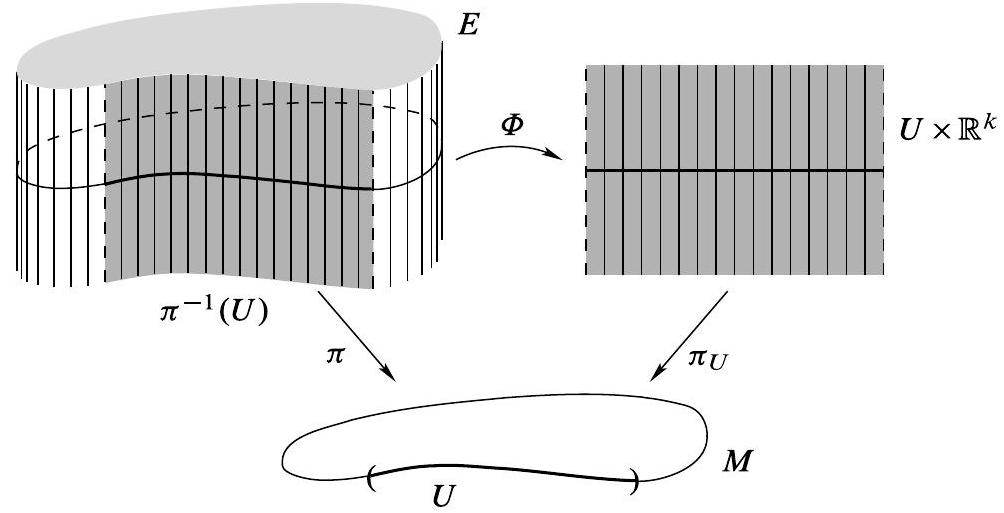
\includegraphics[max width=\textwidth, center]{2025_06_03_90f64b1a1e243cccc2e0g-268}

Fig. 10.1 A local trivialization of a vector bundle\\
(ii) For each $p \in M$, there exist a neighborhood $U$ of $p$ in $M$ and a homeomorphism $\Phi: \pi^{-1}(U) \rightarrow U \times \mathbb{R}^{k}$ (called a local trivialization of $E$ over $U$ ), satisfying the following conditions (Fig. 10.1):

\begin{itemize}
  \item $\pi_{U} \circ \Phi=\pi$ (where $\pi_{U}: U \times \mathbb{R}^{k} \rightarrow U$ is the projection);
  \item for each $q \in U$, the restriction of $\Phi$ to $E_{q}$ is a vector space isomorphism from $E_{q}$ to $\{q\} \times \mathbb{R}^{k} \cong \mathbb{R}^{k}$.\\
If $M$ and $E$ are smooth manifolds with or without boundary, $\pi$ is a smooth map, and the local trivializations can be chosen to be diffeomorphisms, then $E$ is called a smooth vector bundle. In this case, we call any local trivialization that is a diffeomorphism onto its image a smooth local trivialization.
\end{itemize}

A rank-1 vector bundle is often called a (real) line bundle. Complex vector bundles are defined similarly, with "real vector space" replaced by "complex vector space" and $\mathbb{R}^{k}$ replaced by $\mathbb{C}^{k}$ in the definition. We have no need to treat complex vector bundles in this book, so all of our vector bundles are understood without further comment to be real.

The space $E$ is called the total space of the bundle, $M$ is called its base, and $\pi$ is its projection. Depending on what we wish to emphasize, we sometimes omit some of the ingredients from the notation, and write " $E$ is a vector bundle over $M$," or " $E \rightarrow M$ is a vector bundle," or " $\pi: E \rightarrow M$ is a vector bundle."

\begin{itemize}
  \item Exercise 10.1. Suppose $E$ is a smooth vector bundle over M. Show that the projection map $\pi: E \rightarrow M$ is a surjective smooth submersion.
\end{itemize}

If there exists a local trivialization of $E$ over all of $M$ (called a global trivialization of $\boldsymbol{E}$ ), then $E$ is said to be a trivial bundle. In this case, $E$ itself is homeomorphic to the product space $M \times \mathbb{R}^{k}$. If $E \rightarrow M$ is a smooth bundle that admits a smooth global trivialization, then we say that $E$ is smoothly trivial. In this case $E$ is diffeomorphic to $M \times \mathbb{R}^{k}$, not just homeomorphic. For brevity, when we say that a smooth bundle is trivial, we always understand this to mean smoothly trivial, not just trivial in the topological sense.\\
$\Phi_{\alpha}:$

$$
\pi^{-1}\left(V_{p}\right) \xrightarrow{\Phi_{\alpha}} V_{p} \times \mathbb{R}^{k} \xrightarrow{\varphi_{p} \times \mathrm{Id}_{\mathbb{R}^{k}}} \widehat{V}_{p} \times \mathbb{R}^{k}
$$

We will show that the collection of all such charts $\left\{\left(\pi^{-1}\left(V_{p}\right), \widetilde{\varphi}_{p}\right): p \in M\right\}$ satisfies the conditions of the smooth manifold chart lemma (Lemma 1.35) or its counterpart for manifolds with boundary (Exercise 1.43), and therefore gives $E$ the structure of a smooth manifold with or without boundary.

As a composition of bijective maps, $\widetilde{\varphi}_{p}$ is bijective onto an open subset of either $\mathbb{R}^{n} \times \mathbb{R}^{k}=\mathbb{R}^{n+k}$ or $\mathbb{H}^{n} \times \mathbb{R}^{k} \approx \mathbb{H}^{n+k}$. For any $p, q \in M$, it is easy to check that

$$
\widetilde{\varphi}_{p}\left(\pi^{-1}\left(V_{p}\right) \cap \pi^{-1}\left(V_{q}\right)\right)=\varphi_{p}\left(V_{p} \cap V_{q}\right) \times \mathbb{R}^{k}
$$

which is open because $\varphi_{p}$ is a homeomorphism onto an open subset of $\mathbb{R}^{n}$ or $\mathbb{H}^{n}$. Wherever two such charts overlap, we have

$$
\widetilde{\varphi}_{p} \circ \widetilde{\varphi}_{q}^{-1}=\left(\varphi_{p} \times \operatorname{Id}_{\mathbb{R}^{k}}\right) \circ \Phi_{\alpha} \circ \Phi_{\beta}^{-1} \circ\left(\varphi_{q} \times \operatorname{Id}_{\mathbb{R}^{k}}\right)^{-1}
$$

Since $\varphi_{p} \times \operatorname{Id}_{\mathbb{R}^{k}}, \varphi_{q} \times \operatorname{Id}_{\mathbb{R}^{k}}$, and $\Phi_{\alpha} \circ \Phi_{\beta}^{-1}$ are diffeomorphisms, the composition is a diffeomorphism. Thus, conditions (i)-(iii) of Lemma 1.35 are satisfied. Because the open cover $\left\{V_{p}: p \in M\right\}$ has a countable subcover, (iv) is satisfied as well.

To check the Hausdorff condition (v), just note that any two points in the same space $E_{p}$ lie in one of the charts we have constructed; while if $\xi \in E_{p}$ and $\eta \in E_{q}$ with $p \neq q$, we can choose $V_{p}$ and $V_{q}$ to be disjoint neighborhoods of $p$ and $q$, so that the sets $\pi^{-1}\left(V_{p}\right)$ and $\pi^{-1}\left(V_{q}\right)$ are disjoint coordinate neighborhoods containing $\xi$ and $\eta$, respectively. Thus we have given $E$ the structure of a smooth manifold with or without boundary.

With respect to this structure, each of the maps $\Phi_{\alpha}$ is a diffeomorphism, because in terms of the coordinate charts $\left(\pi^{-1}\left(V_{p}\right), \widetilde{\varphi}_{p}\right)$ for $E$ and $\left(V_{p} \times \mathbb{R}^{k}, \varphi_{p} \times \operatorname{Id}_{\mathbb{R}^{k}}\right)$ for $V_{p} \times \mathbb{R}^{k}$, the coordinate representation of $\Phi_{\alpha}$ is the identity map. The coordinate representation of $\pi$, with respect to the same chart for $E$ and the chart $\left(V_{p}, \varphi_{p}\right)$ for $M$, is $\pi(x, v)=x$, so $\pi$ is smooth as well. Because each $\Phi_{\alpha}$ maps $E_{p}$ to $\{p\} \times \mathbb{R}^{k}$, it is immediate that $\pi_{1} \circ \Phi_{\alpha}=\pi$, and $\Phi_{\alpha}$ is linear on fibers by hypothesis. Thus, $\Phi_{\alpha}$ satisfies all the conditions for a smooth local trivialization.

The fact that this is the unique such smooth structure follows easily from the requirement that the maps $\Phi_{\alpha}$ be diffeomorphisms onto their images: any smooth structure satisfying the same conditions must include all of the charts we constructed, so it is equal to this one.

Here are some examples showing how the chart lemma can be used to construct new vector bundles from old ones.

Example 10.7 (Whitney Sums). Given a smooth manifold $M$ and smooth vector bundles $E^{\prime} \rightarrow M$ and $E^{\prime \prime} \rightarrow M$ of ranks $k^{\prime}$ and $k^{\prime \prime}$, respectively, we will construct a new vector bundle over $M$ called the Whitney sum of $\boldsymbol{E}^{\prime}$ and $\boldsymbol{E}^{\prime \prime}$, whose fiber at each $p \in M$ is the direct sum $E_{p}^{\prime} \oplus E_{p}^{\prime \prime}$. The total space is defined as $E^{\prime} \oplus E^{\prime \prime}=$ $\bigsqcup_{p \in M}\left(E_{p}^{\prime} \oplus E_{p}^{\prime \prime}\right)$, with the obvious projection $\pi: E^{\prime} \oplus E^{\prime \prime} \rightarrow M$. For each $p \in M$,\\
choose a neighborhood $U$ of $p$ small enough that there exist local trivializations $\left(U, \Phi^{\prime}\right)$ of $E^{\prime}$ and $\left(U, \Phi^{\prime \prime}\right)$ of $E^{\prime \prime}$, and define $\Phi: \pi^{-1}(U) \rightarrow U \times \mathbb{R}^{k^{\prime}+k^{\prime \prime}}$ by

$$
\Phi\left(v^{\prime}, v^{\prime \prime}\right)=\left(\pi^{\prime}\left(v^{\prime}\right),\left(\pi_{\mathbb{R}^{k^{\prime}}} \circ \Phi^{\prime}\left(v^{\prime}\right), \pi_{\mathbb{R}^{k^{\prime \prime}}} \circ \Phi^{\prime \prime}\left(v^{\prime \prime}\right)\right)\right)
$$

Suppose we are given another such pair of local trivializations $\left(\tilde{U}, \tilde{\Phi}^{\prime}\right)$ and $\left(\tilde{U}, \widetilde{\Phi}^{\prime \prime}\right)$. Let $\tau^{\prime}:(U \cap \tilde{U}) \rightarrow \mathrm{GL}\left(k^{\prime}, \mathbb{R}\right)$ and $\tau^{\prime \prime}:(U \cap \tilde{U}) \rightarrow \mathrm{GL}\left(k^{\prime \prime}, \mathbb{R}\right)$ be the corresponding transition functions. Then the transition function for $E^{\prime} \oplus E^{\prime \prime}$ has the form

$$
\widetilde{\Phi} \circ \Phi^{-1}\left(p,\left(v^{\prime}, v^{\prime \prime}\right)\right)=\left(p, \tau(p)\left(v^{\prime}, v^{\prime \prime}\right)\right)
$$

where $\tau(p)=\tau^{\prime}(p) \oplus \tau^{\prime \prime}(p) \in \mathrm{GL}\left(k^{\prime}+k^{\prime \prime}, \mathbb{R}\right)$ is the block diagonal matrix

$$
\left(\begin{array}{cc}
\tau^{\prime}(p) & 0 \\
0 & \tau^{\prime \prime}(p)
\end{array}\right)
$$

Because this depends smoothly on $p$, it follows from the chart lemma that $E^{\prime} \oplus E^{\prime \prime}$ is a smooth vector bundle over $M$. //

Example 10.8 (Restriction of a Vector Bundle). Suppose $\pi: E \rightarrow M$ is a rank- $k$ vector bundle and $S \subseteq M$ is any subset. We define the restriction of $\boldsymbol{E}$ to $\boldsymbol{S}$ to be the set $\left.E\right|_{S}=\bigcup_{p \in S} E_{p}$, with the projection $\left.E\right|_{S} \rightarrow S$ obtained by restricting $\pi$. If $\Phi: \pi^{-1}(U) \rightarrow U \times \mathbb{R}^{k}$ is a local trivialization of $E$ over $U \subseteq M$, it restricts to a bijective map $\left.\Phi\right|_{U}:\left(\left.\pi\right|_{S}\right)^{-1}(U \cap S) \rightarrow(U \cap S) \times \mathbb{R}^{k}$, and it is easy to check that these form local trivializations for a vector bundle structure on $\left.E\right|_{S}$. If $E$ is a smooth vector bundle and $S \subseteq M$ is an immersed or embedded submanifold, it follows easily from the chart lemma that $\left.E\right|_{S}$ is a smooth vector bundle. In particular, if $S \subseteq M$ is a smooth (embedded or immersed) submanifold, then the restricted bundle $\left.T M\right|_{S}$ is called the ambient tangent bundle over M.

\section*{Local and Global Sections of Vector Bundles}
Let $\pi: E \rightarrow M$ be a vector bundle. A section of $\boldsymbol{E}$ (sometimes called a cross section) is a section of the map $\pi$, that is, a continuous map $\sigma: M \rightarrow E$ satisfying $\pi \circ \sigma=\operatorname{Id}_{M}$. This means that $\sigma(p)$ is an element of the fiber $E_{p}$ for each $p \in M$.

More generally, a local section of $\boldsymbol{E}$ is a continuous map $\sigma: U \rightarrow E$ defined on some open subset $U \subseteq M$ and satisfying $\pi \circ \sigma=\operatorname{Id}_{U}$ (see Fig. 10.3). To emphasize the distinction, a section defined on all of $M$ is sometimes called a global section. Note that a local section of $E$ over $U \subseteq M$ is the same as a global section of the restricted bundle $\left.E\right|_{U}$. If $M$ is a smooth manifold with or without boundary and $E$ is a smooth vector bundle, a smooth (local or global) section of $\boldsymbol{E}$ is one that is a smooth map from its domain to $E$.

Just as with vector fields, for some purposes it is useful also to consider maps that would be sections except that they might not be continuous. Thus, we define a rough (local or global) section of $\boldsymbol{E}$ over a set $U \subseteq M$ to be a map $\sigma: U \rightarrow E$\\
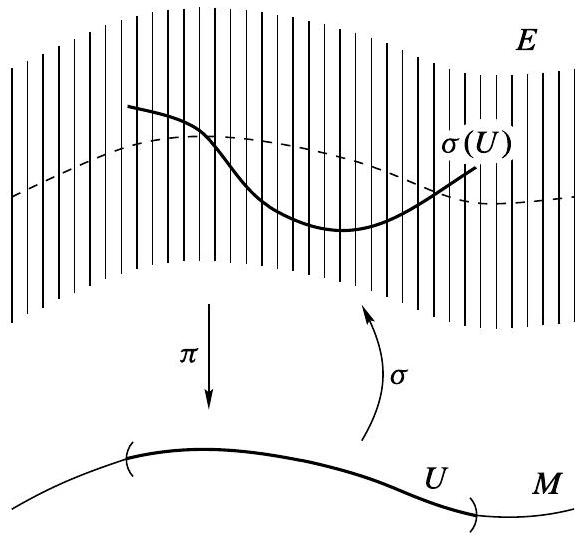
\includegraphics[max width=\textwidth, center]{2025_06_03_90f64b1a1e243cccc2e0g-274}

Fig. 10.3 A local section of a vector bundle\\
(not necessarily continuous) such that $\pi \circ \sigma=\mathrm{Id}_{U}$. A "section" without further qualification always means a continuous section.

The zero section of $\boldsymbol{E}$ is the global section $\zeta: M \rightarrow E$ defined by

$$
\zeta(p)=0 \in E_{p} \text { for each } p \in M .
$$

As in the case of vector fields, the support of a section $\sigma$ is the closure of the set $\{p \in M: \sigma(p) \neq 0\}$.

Exercise 10.9. Show that the zero section of every vector bundle is continuous, and the zero section of every smooth vector bundle is smooth. [Hint: consider $\Phi \circ \zeta$, where $\Phi$ is a local trivialization.]

Example 10.10 (Sections of Vector Bundles). Suppose $M$ is a smooth manifold with or without boundary.\\
(a) Sections of $T M$ are vector fields on $M$.\\
(b) Given an immersed submanifold $S \subseteq M$ with or without boundary, a section of the ambient tangent bundle $\left.T M\right|_{S} \rightarrow S$ is called a vector field along $S$. It is a continuous map $X: S \rightarrow T M$ such that $X_{p} \in T_{p} M$ for each $p \in S$. This is different from a vector field on $S$, which satisfies $X_{p} \in T_{p} S$ at each point.\\
(c) If $E=M \times \mathbb{R}^{k}$ is a product bundle, there is a natural one-to-one correspondence between sections of $E$ and continuous functions from $M$ to $\mathbb{R}^{k}$ : a continuous function $F: M \rightarrow \mathbb{R}^{k}$ determines a section $\widetilde{F}: M \rightarrow M \times \mathbb{R}^{k}$ by $\widetilde{F}(x)=(x, F(x))$, and vice versa. If $M$ is a smooth manifold with or without boundary, then the section $\widetilde{F}$ is smooth if and only if $F$ is.\\
(d) The correspondence in the preceding paragraph yields a natural identification between the space $C^{\infty}(M)$ and the space of smooth sections of the trivial line bundle $M \times \mathbb{R} \rightarrow M$.

If $E \rightarrow M$ is a smooth vector bundle, the set of all smooth global sections of $E$ is a vector space under pointwise addition and scalar multiplication:

$$
\left(c_{1} \sigma_{1}+c_{2} \sigma_{2}\right)(p)=c_{1} \sigma_{1}(p)+c_{2} \sigma_{2}(p) .
$$

This vector space is usually denoted by $\Gamma(E)$. (For particular vector bundles, we will often introduce specialized notations for their spaces of sections, such as the notation $\mathfrak{X}(M)$ introduced in Chapter 8 for the space of smooth sections of $T M$.)

Just like smooth vector fields, smooth sections of a smooth bundle $E \rightarrow M$ can be multiplied by smooth real-valued functions: if $f \in C^{\infty}(M)$ and $\sigma \in \Gamma(E)$, we obtain a new section $f \sigma$ defined by

$$
(f \sigma)(p)=f(p) \sigma(p) .
$$

\begin{itemize}
  \item Exercise 10.11. Let $E \rightarrow M$ be a smooth vector bundle.\\
(a) Show that if $\sigma, \tau \in \Gamma(E)$ and $f, g \in C^{\infty}(M)$, then $f \sigma+g \tau \in \Gamma(E)$.\\
(b) Show that $\Gamma(E)$ is a module over the ring $C^{\infty}(M)$.
\end{itemize}

Lemma 10.12 (Extension Lemma for Vector Bundles). Let $\pi: E \rightarrow M$ be a smooth vector bundle over a smooth manifold $M$ with or without boundary. Suppose $A$ is a closed subset of $M$, and $\sigma: A \rightarrow E$ is a section of $\left.E\right|_{A}$ that is smooth in the sense that $\sigma$ extends to a smooth local section of $E$ in a neighborhood of each point. For each open subset $U \subseteq M$ containing $A$, there exists a global smooth section $\widetilde{\sigma} \in \Gamma(E)$ such that $\left.\widetilde{\sigma}\right|_{A}=\sigma$ and $\operatorname{supp} \widetilde{\sigma} \subseteq U$.

\begin{itemize}
  \item Exercise 10.13. Prove the preceding lemma.
  \item Exercise 10.14. Let $\pi: E \rightarrow M$ be a smooth vector bundle. Show that each element of $E$ is in the image of a smooth global section.
\end{itemize}

\section*{Local and Global Frames}
The concept of local frames that we introduced in Chapter 8 extends readily to vector bundles. Let $E \rightarrow M$ be a vector bundle. If $U \subseteq M$ is an open subset, a $k$ tuple of local sections $\left(\sigma_{1}, \ldots, \sigma_{k}\right)$ of $E$ over $U$ is said to be linearly independent if their values $\left(\sigma_{1}(p), \ldots, \sigma_{k}(p)\right)$ form a linearly independent $k$-tuple in $E_{p}$ for each $p \in U$. Similarly, they are said to span $\boldsymbol{E}$ if their values span $E_{p}$ for each $p \in U$. A local frame for $\boldsymbol{E}$ over $\boldsymbol{U}$ is an ordered $k$-tuple ( $\sigma_{1}, \ldots, \sigma_{k}$ ) of linearly independent local sections over $U$ that span $E$; thus $\left(\sigma_{1}(p), \ldots, \sigma_{k}(p)\right)$ is a basis for the fiber $E_{p}$ for each $p \in U$. It is called a global frame if $U=M$. If $E \rightarrow M$ is a smooth vector bundle, a local or global frame is a smooth frame if each $\sigma_{i}$ is a smooth section. We often denote a frame ( $\sigma_{1}, \ldots, \sigma_{k}$ ) by ( $\sigma_{i}$ ).

The (local or global) frames for $M$ that we defined in Chapter 8 are, in our new terminology, frames for the tangent bundle. We use both terms interchangeably depending on context: "frame for $M$ " and "frame for $T M$ " mean the same thing.

The next proposition is an analogue for vector bundles of Proposition 8.11.

Proposition 10.15 (Completion of Local Frames for Vector Bundles). Suppose $\pi: E \rightarrow M$ is a smooth vector bundle of rank $k$.\\
(a) If $\left(\sigma_{1}, \ldots, \sigma_{m}\right)$ is a linearly independent $m$-tuple of smooth local sections of $E$ over an open subset $U \subseteq M$, with $1 \leq m<k$, then for each $p \in U$ there exist smooth sections $\sigma_{m+1}, \ldots, \sigma_{k}$ defined on some neighborhood $V$ of $p$ such that ( $\sigma_{1}, \ldots, \sigma_{k}$ ) is a smooth local frame for $E$ over $U \cap V$.\\
(b) If $\left(v_{1}, \ldots, v_{m}\right)$ is a linearly independent $m$-tuple of elements of $E_{p}$ for some $p \in M$, with $1 \leq m \leq k$, then there exists a smooth local frame ( $\sigma_{i}$ ) for $E$ over some neighborhood of $p$ such that $\sigma_{i}(p)=v_{i}$ for $i=1, \ldots, m$.\\
(c) If $A \subseteq M$ is a closed subset and ( $\tau_{1}, \ldots, \tau_{k}$ ) is a linearly independent $k$-tuple of sections of $\left.E\right|_{A}$ that are smooth in the sense described in Lemma 10.12, then there exists a smooth local frame ( $\sigma_{1}, \ldots, \sigma_{k}$ ) for $E$ over some neighborhood of $A$ such that $\left.\sigma_{i}\right|_{A}=\tau_{i}$ for $i=1, \ldots, k$.

\begin{itemize}
  \item Exercise 10.16. Prove the preceding proposition.
\end{itemize}

Local frames for a vector bundle are intimately connected with local trivializations, as the next two examples show.

Example 10.17 (A Global Frame for a Product Bundle). If $E=M \times \mathbb{R}^{k} \rightarrow M$ is a product bundle, the standard basis $\left(e_{1}, \ldots, e_{k}\right)$ for $\mathbb{R}^{k}$ yields a global frame $\left(\tilde{e}_{i}\right)$ for $E$, defined by $\tilde{e}_{i}(p)=\left(p, e_{i}\right)$. If $M$ is a smooth manifold with or without boundary, then this global frame is smooth.

Example 10.18 (Local Frames Associated with Local Trivializations). Suppose $\pi: E \rightarrow M$ is a smooth vector bundle. If $\Phi: \pi^{-1}(U) \rightarrow U \times \mathbb{R}^{k}$ is a smooth local trivialization of $E$, we can use the same idea as in the preceding example to construct a local frame for $E$ over $U$. Define maps $\sigma_{1}, \ldots, \sigma_{k}: U \rightarrow E$ by $\sigma_{i}(p)=\Phi^{-1}\left(p, e_{i}\right)=\Phi^{-1} \circ \tilde{e}_{i}(p):$\\
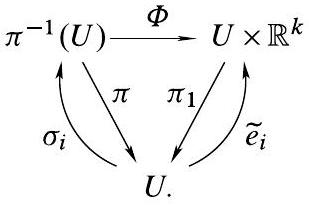
\includegraphics[max width=\textwidth, center]{2025_06_03_90f64b1a1e243cccc2e0g-276}

Then $\sigma_{i}$ is smooth because $\Phi$ is a diffeomorphism, and the fact that $\pi_{1} \circ \Phi=\pi$ implies that

$$
\pi \circ \sigma_{i}(p)=\pi \circ \Phi^{-1}\left(p, e_{i}\right)=\pi_{1}\left(p, e_{i}\right)=p,
$$

so $\sigma_{i}$ is a section. To see that $\left(\sigma_{i}(p)\right)$ forms a basis for $E_{p}$, just note that $\Phi$ restricts to an isomorphism from $E_{p}$ to $\{p\} \times \mathbb{R}^{k}$, and $\Phi\left(\sigma_{i}(p)\right)=\left(p, e_{i}\right)$, so $\Phi$ takes $\left(\sigma_{i}(p)\right)$ to the standard basis for $\{p\} \times \mathbb{R}^{k} \cong \mathbb{R}^{k}$. We say that this local frame $\left(\sigma_{i}\right)$ is associated with $\boldsymbol{\Phi}$.

Proposition 10.19. Every smooth local frame for a smooth vector bundle is associated with a smooth local trivialization as in Example 10.18.

Proof. Suppose $E \rightarrow M$ is a smooth vector bundle and $\left(\sigma_{i}\right)$ is a smooth local frame for $E$ over an open subset $U \subseteq M$. We define a map $\Psi: U \times \mathbb{R}^{k} \rightarrow \pi^{-1}(U)$ by

$$
\Psi\left(p,\left(v^{1}, \ldots, v^{k}\right)\right)=v^{i} \sigma_{i}(p)
$$

The fact that $\left(\sigma_{i}(p)\right)$ forms a basis for $E_{p}$ at each $p \in U$ implies that $\Psi$ is bijective, and an easy computation shows that $\sigma_{i}=\Psi \circ \tilde{e}_{i}$. Thus, if we can show that $\Psi$ is a diffeomorphism, then $\Psi^{-1}$ will be a smooth local trivialization whose associated local frame is $\left(\sigma_{i}\right)$.

Since $\Psi$ is bijective, to show that it is a diffeomorphism it suffices to show that it is a local diffeomorphism. Given $q \in U$, we can choose a neighborhood $V$ of $q$ in $M$ over which there exists a smooth local trivialization $\Phi: \pi^{-1}(V) \rightarrow V \times \mathbb{R}^{k}$, and by shrinking $V$ if necessary we may assume that $V \subseteq U$. Since $\Phi$ is a diffeomorphism, if we can show that $\left.\Phi \circ \Psi\right|_{V \times \mathbb{R}^{k}}$ is a diffeomorphism from $V \times \mathbb{R}^{k}$ to itself, it follows that $\Psi$ restricts to a diffeomorphism from $V \times \mathbb{R}^{k}$ to $\pi^{-1}(V)$ :\\
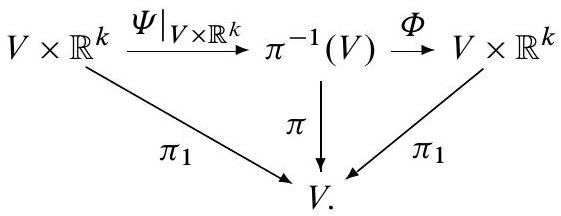
\includegraphics[max width=\textwidth, center]{2025_06_03_90f64b1a1e243cccc2e0g-277}

For each of our smooth sections $\sigma_{i}$, the composite map $\left.\Phi \circ \sigma_{i}\right|_{V}: V \rightarrow V \times \mathbb{R}^{k}$ is smooth, and thus there are smooth functions $\sigma_{i}^{1}, \ldots, \sigma_{i}^{k}: V \rightarrow \mathbb{R}$ such that

$$
\Phi \circ \sigma_{i}(p)=\left(p,\left(\sigma_{i}^{1}(p), \ldots, \sigma_{i}^{k}(p)\right)\right) .
$$

On $V \times \mathbb{R}^{k}$, therefore,

$$
\Phi \circ \Psi\left(p,\left(v^{1}, \ldots, v^{k}\right)\right)=\left(p,\left(v^{i} \sigma_{i}^{1}(p), \ldots, v^{i} \sigma_{i}^{k}(p)\right)\right),
$$

which is clearly smooth.\\
To show that $(\Phi \circ \Psi)^{-1}$ is smooth, note that the matrix $\left(\sigma_{i}^{j}(p)\right)$ is invertible for each $p$, because $\left(\sigma_{i}(p)\right)$ is a basis for $E_{p}$. Let $\left(\tau_{i}^{j}(p)\right)$ denote the inverse matrix. Because matrix inversion is a smooth map from $\operatorname{GL}(k, \mathbb{R})$ to itself, the functions $\tau_{i}^{j}$ are smooth. It follows from the computations in the preceding paragraph that

$$
(\Phi \circ \Psi)^{-1}\left(p,\left(w^{1}, \ldots, w^{k}\right)\right)=\left(p,\left(w^{i} \tau_{i}^{1}(p), \ldots, w^{i} \tau_{i}^{k}(p)\right)\right),
$$

which is also smooth.\\
Corollary 10.20. A smooth vector bundle is smoothly trivial if and only if it admits a smooth global frame.

Proof. Example 10.18 and Proposition 10.19 show that there is a smooth local trivialization over an open subset $U \subseteq M$ if and only if there is a smooth local frame over $U$. The corollary is just the special case of this statement when $U=M$.

When applied to the tangent bundle of a smooth manifold $M$, this corollary says that $T M$ is trivial if and only if $M$ is parallelizable. (Recall that in Chapter 8 we\\
defined a parallelizable manifold to be one that admits a smooth global frame for its tangent bundle.)

Corollary 10.21. Let $\pi: E \rightarrow M$ be a smooth vector bundle of rank $k$, let ( $V, \varphi$ ) be a smooth chart on $M$ with coordinate functions ( $x^{i}$ ), and suppose there exists a smooth local frame $\left(\sigma_{i}\right)$ for $E$ over $V$. Define $\tilde{\varphi}: \pi^{-1}(V) \rightarrow \varphi(V) \times \mathbb{R}^{k}$ by

$$
\widetilde{\varphi}\left(v^{i} \sigma_{i}(p)\right)=\left(x^{1}(p), \ldots, x^{n}(p), v^{1}, \ldots, v^{k}\right)
$$

Then $\left(\pi^{-1}(V), \widetilde{\varphi}\right)$ is a smooth coordinate chart for $E$.\\
Proof. Just check that $\widetilde{\varphi}$ is equal to the composition $\left(\varphi \times \operatorname{Id}_{\mathbb{R}^{k}}\right) \circ \Phi$, where $\Phi$ is the local trivialization associated with ( $\sigma_{i}$ ). As a composition of diffeomorphisms, it is a diffeomorphism.

Just as smoothness of vector fields can be characterized in terms of their component functions in any smooth chart, smoothness of sections of vector bundles can be characterized in terms of local frames. Suppose ( $\sigma_{i}$ ) is a smooth local frame for $E$ over some open subset $U \subseteq M$. If $\tau: M \rightarrow E$ is a rough section, the value of $\tau$ at an arbitrary point $p \in U$ can be written $\tau(p)=\tau^{i}(p) \sigma_{i}(p)$ for some uniquely determined numbers $\left(\tau^{1}(p), \ldots, \tau^{n}(p)\right)$. This defines $k$ functions $\tau^{i}: U \rightarrow \mathbb{R}$, called the component functions of $\tau$ with respect to the given local frame.

Proposition 10.22 (Local Frame Criterion for Smoothness). Let $\pi: E \rightarrow M$ be a smooth vector bundle, and let $\tau: M \rightarrow E$ be a rough section. If $\left(\sigma_{i}\right)$ is a smooth local frame for $E$ over an open subset $U \subseteq M$, then $\tau$ is smooth on $U$ if and only if its component functions with respect to ( $\sigma_{i}$ ) are smooth.\\
Proof. Let $\Phi: \pi^{-1}(U) \rightarrow U \times \mathbb{R}^{k}$ be the local trivialization associated with the local frame ( $\sigma_{i}$ ). Because $\Phi$ is a diffeomorphism, $\tau$ is smooth on $U$ if and only if the composite map $\Phi \circ \tau$ is smooth on $U$. It is straightforward to check that $\Phi \circ \tau(p)=\left(p,\left(\tau^{1}(p), \ldots, \tau^{k}(p)\right)\right)$, where $\left(\tau^{i}\right)$ are the component functions of $\tau$ with respect to $\left(\sigma_{i}\right)$, so $\Phi \circ \tau$ is smooth if and only if the component functions $\tau^{i}$ are smooth.

\begin{itemize}
  \item Exercise 10.23. Let $E \rightarrow M$ be a vector bundle. Show that a rough section of $E$ is continuous if and only if its component functions in each local frame are continuous.
\end{itemize}

Proposition 10.22 applies equally well to local sections, since a local section of $E$ over an open subset $V \subseteq M$ is a global section of the restricted bundle $\left.E\right|_{V}$.

The correspondence between local frames and local trivializations leads to the following uniqueness result characterizing the smooth structure on the tangent bundle of a smooth manifold.

Proposition 10.24 (Uniqueness of the Smooth Structure on TM). Let $M$ be a smooth $n$-manifold with or without boundary. The topology and smooth structure on TM constructed in Proposition 3.18 are the unique ones with respect to which $\pi: T M \rightarrow M$ is a smooth vector bundle with the given vector space structure on the fibers, and such that all coordinate vector fields are smooth local sections.

Proof. Suppose TM is endowed with some topology and smooth structure making it into a smooth vector bundle with the given properties. If $(U, \varphi)$ is any smooth chart for $M$, the corresponding coordinate frame $\left(\partial / \partial x^{i}\right)$ is a smooth local frame over $U$, so by Proposition 10.19 there is a smooth local trivialization $\Phi: \pi^{-1}(U) \rightarrow U \times \mathbb{R}^{n}$ associated with this local frame. Referring back to the construction of Example 10.18, we see that this local trivialization is none other than the map $\Phi$ constructed in Proposition 10.4. It follows from Corollary 10.21 that the natural coordinate chart $\widetilde{\varphi}=\left(\varphi \times \mathrm{Id}_{\mathbb{R}^{n}}\right) \circ \Phi$ belongs to the given smooth structure. Thus, the given smooth structure is equal to the one constructed in Proposition 3.18.

\section*{Bundle Homomorphisms}
If $\pi: E \rightarrow M$ and $\pi^{\prime}: E^{\prime} \rightarrow M^{\prime}$ are vector bundles, a continuous map $F: E \rightarrow E^{\prime}$ is called a bundle homomorphism if there exists a map $f: M \rightarrow M^{\prime}$ satisfying $\pi^{\prime} \circ F=f \circ \pi$,\\
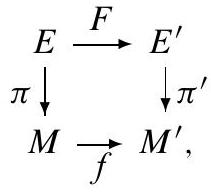
\includegraphics[max width=\textwidth, center]{2025_06_03_90f64b1a1e243cccc2e0g-279}\\
with the property that for each $p \in M$, the restricted map $\left.F\right|_{E_{p}}: E_{p} \rightarrow E_{f(p)}^{\prime}$ is linear. The relationship between $F$ and $f$ is expressed by saying that $\boldsymbol{F}$ covers $\boldsymbol{f}$.

Proposition 10.25. Suppose $\pi: E \rightarrow M$ and $\pi^{\prime}: E \rightarrow M^{\prime}$ are vector bundles and $F: E \rightarrow E^{\prime}$ is a bundle homomorphism covering $f: M \rightarrow M^{\prime}$. Then $f$ is continuous and is uniquely determined by $F$. If the bundles and $F$ are all smooth, then $f$ is smooth as well.

Proof. All of the conclusions follow from the easily verified fact that $f=\pi^{\prime} \circ F \circ \zeta$, where $\zeta: M \rightarrow E$ is the zero section.

A bijective bundle homomorphism $F: E \rightarrow E^{\prime}$ whose inverse is also a bundle homomorphism is called a bundle isomorphism; if $F$ is also a diffeomorphism, it is called a smooth bundle isomorphism. If there exists a (smooth) bundle isomorphism between $E$ and $E^{\prime}$, the two bundles are said to be (smoothly) isomorphic.

In the special case in which both $E$ and $E^{\prime}$ are vector bundles over the same base space $M$, a slightly more restrictive notion of bundle homomorphism is usually more useful. A bundle homomorphism over $\mathbf{M}$ is a bundle homomorphism covering the identity map of $M$, or in other words, a continuous map $F: E \rightarrow E^{\prime}$ such that $\pi^{\prime} \circ F=\pi$,\\
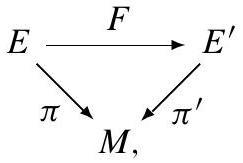
\includegraphics[max width=\textwidth, center]{2025_06_03_90f64b1a1e243cccc2e0g-279(1)}\\
and whose restriction to each fiber is linear. If there exists a bundle homomorphism $F: E \rightarrow E^{\prime}$ over $M$ that is also a (smooth) bundle isomorphism, then we say that\\
$E$ and $E^{\prime}$ are (smoothly) isomorphic over M. The next proposition shows that it is not necessary to check smoothness of the inverse.

Proposition 10.26. Suppose $E$ and $E^{\prime}$ are smooth vector bundles over a smooth manifold $M$ with or without boundary, and $F: E \rightarrow E^{\prime}$ is a bijective smooth bundle homomorphism over M. Then F is a smooth bundle isomorphism.

Proof. Problem 10-11.\\
Exercise 10.27. Show that a smooth rank- $k$ vector bundle over $M$ is smoothly trivial if and only if it is smoothly isomorphic over $M$ to the product bundle $M \times \mathbb{R}^{k}$.

\section*{Example 10.28 (Bundle Homomorphisms).}
(a) If $F: M \rightarrow N$ is a smooth map, the global differential $d F: T M \rightarrow T N$ is a smooth bundle homomorphism covering $F$.\\
(b) If $E \rightarrow M$ is a smooth vector bundle and $S \subseteq M$ is an immersed submanifold with or without boundary, then the inclusion map $\left.E\right|_{S} \hookrightarrow E$ is a smooth bundle homomorphism covering the inclusion of $S$ into $M$.

Suppose $E \rightarrow M$ and $E^{\prime} \rightarrow M$ are smooth vector bundles over a smooth manifold $M$ with or without boundary, and let $\Gamma(E), \Gamma\left(E^{\prime}\right)$ denote their spaces of smooth global sections. If $F: E \rightarrow E^{\prime}$ is a smooth bundle homomorphism over $M$, then composition with $F$ induces a map $\widetilde{F}: \Gamma(E) \rightarrow \Gamma\left(E^{\prime}\right)$ as follows:

$$
\tilde{F}(\sigma)(p)=(F \circ \sigma)(p)=F(\sigma(p)) .
$$

It is easy to check that $\widetilde{F}(\sigma)$ is a section of $E^{\prime}$, and it is smooth by composition.\\
Because a bundle homomorphism is linear on fibers, the resulting map $\widetilde{F}$ on sections is linear over $\mathbb{R}$. In fact, it satisfies a stronger linearity property. A map $\mathcal{F}: \Gamma(E) \rightarrow \Gamma\left(E^{\prime}\right)$ is said to be linear over $\boldsymbol{C}^{\infty}(\boldsymbol{M})$ if for any smooth functions $u_{1}, u_{2} \in C^{\infty}(M)$ and smooth sections $\sigma_{1}, \sigma_{2} \in \Gamma(E)$,

$$
\mathscr{F}\left(u_{1} \sigma_{1}+u_{2} \sigma_{2}\right)=u_{1} \mathscr{F}\left(\sigma_{1}\right)+u_{2} \mathscr{F}\left(\sigma_{2}\right) .
$$

It follows easily from the definition (10.5) that the map on sections induced by a smooth bundle homomorphism is linear over $C^{\infty}(M)$. The next lemma shows that the converse is true as well.

Lemma 10.29 (Bundle Homomorphism Characterization Lemma). Let $\pi: E \rightarrow$ $M$ and $\pi^{\prime}: E^{\prime} \rightarrow M$ be smooth vector bundles over a smooth manifold $M$ with or without boundary, and let $\Gamma(E), \Gamma\left(E^{\prime}\right)$ denote their spaces of smooth sections. A map $\mathscr{F}: \Gamma(E) \rightarrow \Gamma\left(E^{\prime}\right)$ is linear over $C^{\infty}(M)$ if and only if there is a smooth bundle homomorphism $F: E \rightarrow E^{\prime}$ over $M$ such that $\mathcal{F}(\sigma)=F \circ \sigma$ for all $\sigma \in \Gamma(E)$.

Proof. We noted above that the map on sections induced by a smooth bundle homomorphism is linear over $C^{\infty}(M)$. Conversely, suppose $\mathcal{F}: \Gamma(E) \rightarrow \Gamma\left(E^{\prime}\right)$ is linear over $C^{\infty}(M)$. First, we show that $\mathcal{F}$ acts locally: if $\sigma_{1} \equiv \sigma_{2}$ in some open subset $U \subseteq M$, then $\mathscr{F}\left(\sigma_{1}\right) \equiv \mathscr{F}\left(\sigma_{2}\right)$ in $U$. Write $\tau=\sigma_{1}-\sigma_{2}$; then by linearity of $\mathscr{F}$, it\\
suffices to assume that $\tau$ vanishes in $U$ and show that $\mathscr{F}(\tau)$ does too. Given $p \in U$, let $\psi \in C^{\infty}(M)$ be a smooth bump function supported in $U$ and equal to 1 at $p$. Because $\psi \tau$ is identically zero on $M$, the fact that $\mathscr{F}$ is linear over $C^{\infty}(M)$ implies

$$
0=\mathscr{F}(\psi \tau)=\psi \mathscr{F}(\tau)
$$

Evaluating at $p$ shows that $\mathscr{F}(\tau)(p)=\psi(p) \mathscr{F}(\tau)(p)=0$; since the same is true for every $p \in U$, the claim follows.

Next we show that $\mathcal{F}$ actually acts pointwise: if $\sigma_{1}(p)=\sigma_{2}(p)$, then $\mathcal{F}\left(\sigma_{1}\right)(p)=\mathcal{F}\left(\sigma_{2}\right)(p)$. Once again, it suffices to assume that $\tau(p)=0$ and show that $\mathcal{F}(\tau)(p)=0$. Let $\left(\sigma_{1}, \ldots, \sigma_{k}\right)$ be a smooth local frame for $E$ in some neighborhood $U$ of $p$, and write $\tau$ in terms of this frame as $\tau=u^{i} \sigma_{i}$ for some smooth functions $u^{i}$ defined in $U$. The fact that $\tau(p)=0$ means that $u^{1}(p)=\cdots=u^{k}(p)=0$. By the extension lemmas for vector bundles and for functions, there exist smooth global sections $\tilde{\sigma}_{i} \in \Gamma(E)$ that agree with $\sigma_{i}$ in a neighborhood of $p$, and smooth functions $\tilde{u}^{i} \in C^{\infty}(M)$ that agree with $u^{i}$ in some neighborhood of $p$. Then since $\tau=\tilde{u}^{i} \tilde{\sigma}_{i}$ on a neighborhood of $p$, we have

$$
\mathscr{F}(\tau)(p)=\mathscr{F}\left(\tilde{u}^{i} \tilde{\sigma}_{i}\right)(p)=\tilde{u}^{i}(p) \mathscr{F}\left(\tilde{\sigma}_{i}\right)(p)=0
$$

Define a bundle homomorphism $F: E \rightarrow E^{\prime}$ as follows. For any $p \in M$ and $v \in E_{p}$, let $F(v)=\mathcal{F}(\tilde{v})(p) \in E_{p}^{\prime}$, where $\widetilde{v}$ is any global smooth section of $E$ such that $\tilde{v}(p)=v$. The discussion above shows that the resulting element of $E_{p}^{\prime}$ is independent of the choice of section. This map $F$ clearly satisfies $\pi^{\prime} \circ F=\pi$, and it is linear on each fiber because of the linearity of $\mathcal{F}$. It also satisfies $F \circ \sigma(p)=$ $\mathcal{F}(\sigma)(p)$ for each $\sigma \in \Gamma(E)$ by definition. It remains only to show that $F$ is smooth. It suffices to show that it is smooth in a neighborhood of each point.

Given $p \in M$, let $\left(\sigma_{i}\right)$ be a smooth local frame for $E$ on some neighborhood of $p$. By the extension lemma, there are global sections $\widetilde{\sigma}_{i}$ that agree with $\sigma_{i}$ in a (smaller) neighborhood $U$ of $p$. Shrinking $U$ further if necessary, we may also assume that there exists a smooth local frame $\left(\sigma_{j}^{\prime}\right)$ for $E^{\prime}$ over $U$. Because $\mathcal{F}$ maps smooth global sections of $E$ to smooth global sections of $E^{\prime}$, there are smooth functions $A_{i}^{j} \in C^{\infty}(U)$ such that $\left.\mathscr{F}\left(\widetilde{\sigma}_{i}\right)\right|_{U}=A_{i}^{j} \sigma_{j}^{\prime}$.

For any $q \in U$ and $v \in E_{q}$, we can write $v=v^{i} \sigma_{i}(q)$ for some real numbers $\left(v^{1}, \ldots, v^{k}\right)$, and then

$$
F\left(v^{i} \sigma_{i}(q)\right)=\mathcal{F}\left(v^{i} \widetilde{\sigma}_{i}\right)(q)=v^{i} \mathcal{F}\left(\widetilde{\sigma}_{i}\right)(q)=v^{i} A_{i}^{j}(q) \sigma_{j}^{\prime}(q),
$$

because $v^{i} \widetilde{\sigma}_{i}$ is a global smooth section of $E$ whose value at $q$ is $v$. If $\Phi$ and $\Phi^{\prime}$ denote the local trivializations of $E$ and $E^{\prime}$ associated with the frames $\left(\sigma_{i}\right)$ and $\left(\sigma_{i}^{\prime}\right)$, respectively, it follows that the composite map $\Phi^{\prime} \circ F \circ \Phi^{-1}: U \times \mathbb{R}^{k} \rightarrow U \times \mathbb{R}^{m}$ has the form

$$
\Phi^{\prime} \circ F \circ \Phi^{-1}\left(q,\left(v^{1}, \ldots, v^{k}\right)\right)=\left(q,\left(A_{i}^{1}(q) v^{i}, \ldots, A_{i}^{m}(q) v^{i}\right)\right)
$$

which is smooth. Because $\Phi$ and $\Phi^{\prime}$ are diffeomorphisms, this shows that $F$ is smooth on $\pi^{-1}(U)$.

Later, after we have developed more tools, we will see many examples of smooth bundle homomorphisms. For now, here are some elementary examples.

\section*{Example 10.30 (Bundle Homomorphisms Over Manifolds).}
(a) If $M$ is a smooth manifold and $f \in C^{\infty}(M)$, the map from $\mathfrak{X}(M)$ to itself defined by $X \mapsto f X$ is linear over $C^{\infty}(M)$ because $f\left(u_{1} X_{1}+u_{2} X_{2}\right)=$ $u_{1} f X_{1}+u_{2} f X_{2}$, and thus defines a smooth bundle homomorphism over $M$ from $T M$ to itself.\\
(b) If $Z$ is a smooth vector field on $\mathbb{R}^{3}$, the cross product with $Z$ defines a map from $\mathfrak{X}\left(\mathbb{R}^{3}\right)$ to itself: $X \mapsto X \times Z$. Since it is linear over $C^{\infty}\left(\mathbb{R}^{3}\right)$ in $X$, it determines a smooth bundle homomorphism over $\mathbb{R}^{3}$ from $T \mathbb{R}^{3}$ to $T \mathbb{R}^{3}$.\\
(c) Given $Z \in \mathfrak{X}\left(\mathbb{R}^{n}\right)$, the Euclidean dot product defines a map $X \mapsto X \cdot Z$ from $\mathfrak{X}\left(\mathbb{R}^{n}\right)$ to $C^{\infty}\left(\mathbb{R}^{n}\right)$, which is linear over $C^{\infty}\left(\mathbb{R}^{n}\right)$ and thus determines a smooth bundle homomorphism over $\mathbb{R}^{n}$ from $T \mathbb{R}^{n}$ to the trivial line bundle $\mathbb{R}^{n} \times \mathbb{R}$.\\
//\\
Because of Lemma 10.29, we usually dispense with the notation $\widetilde{F}$ and use the same symbol for both a bundle homomorphism $F: E \rightarrow E^{\prime}$ over $M$ and the linear map $F: \Gamma(E) \rightarrow \Gamma\left(E^{\prime}\right)$ that it induces on sections, and we refer to a map of either of these types as a bundle homomorphism. Because the action on sections is obtained simply by applying the bundle homomorphism pointwise, this should cause no confusion. In fact, we have been doing the same thing all along in certain circumstances. For example, if $a \in \mathbb{R}$, we use the same notation $X \mapsto a X$ to denote both the operation of multiplying vectors in each tangent space $T_{p} M$ by $a$, and the operation of multiplying vector fields by $a$. Because multiplying by $a$ is a bundle homomorphism from $T M$ to itself, there is no ambiguity about what is meant.

It should be noted that most maps that involve differentiation are not bundle homomorphism. For example, if $X$ is a smooth vector field on a smooth manifold $M$, the Lie derivative operator $\mathscr{L}_{X}: \mathfrak{X}(M) \rightarrow \mathfrak{X}(M)$ is not a bundle homomorphism from the tangent bundle to itself, because it is not linear over $C^{\infty}(M)$. As a rule of thumb, a linear map that takes smooth sections of one bundle to smooth sections of another is likely to be a bundle homomorphism if it acts pointwise, but not if it involves differentiation.

\section*{Subbundles}
Given a vector bundle $\pi_{E}: E \rightarrow$ M, a subbundle of $\boldsymbol{E}$ (see Fig. 10.4) is a vector bundle $\pi_{D}: D \rightarrow M$, in which $D$ is a topological subspace of $E$ and $\pi_{D}$ is the restriction of $\pi_{E}$ to $D$, such that for each $p \in M$, the subset $D_{p}=D \cap E_{p}$ is a linear subspace of $E_{p}$, and the vector space structure on $D_{p}$ is the one inherited from $E_{p}$. Note that the condition that $D$ be a vector bundle over $M$ implies that all of the fibers $D_{p}$ must be nonempty and have the same dimension. If $E \rightarrow M$ is a smooth bundle, then a subbundle of $E$ is called a smooth subbundle if it is a smooth vector bundle and an embedded submanifold with or without boundary in $E$.\\
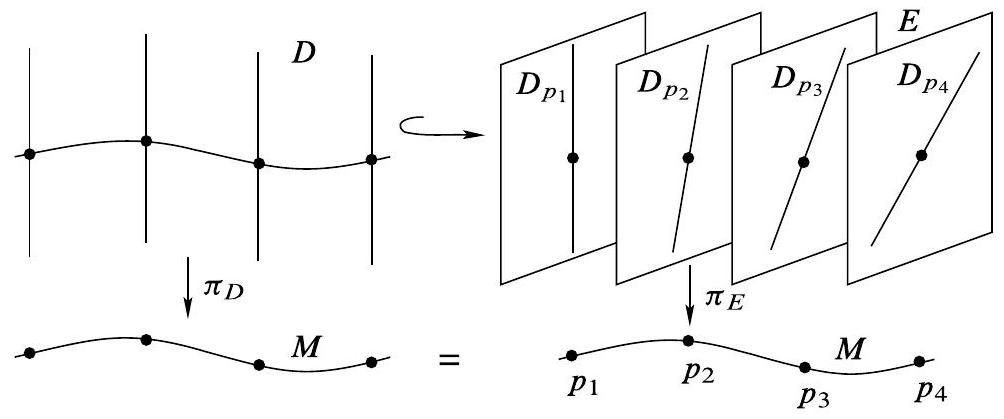
\includegraphics[max width=\textwidth, center]{2025_06_03_90f64b1a1e243cccc2e0g-283}

Fig. 10.4 A subbundle of a vector bundle

\begin{itemize}
  \item Exercise 10.31. Given a smooth vector bundle $E \rightarrow M$ and a smooth subbundle $D \subseteq E$, show that the inclusion map $\iota: D \hookrightarrow E$ is a smooth bundle homomorphism over $M$.
\end{itemize}

The following lemma gives a convenient condition for checking that a union of subspaces $\left\{D_{p} \subseteq E_{p}: p \in M\right\}$ is a smooth subbundle.

Lemma 10.32 (Local Frame Criterion for Subbundles). Let $\pi: E \rightarrow M$ be a smooth vector bundle, and suppose that for each $p \in M$ we are given an $m$ dimensional linear subspace $D_{p} \subseteq E_{p}$. Then $D=\bigcup_{p \in M} D_{p} \subseteq E$ is a smooth subbundle of $E$ if and only if the following condition is satisfied:

\begin{displayquote}
Each point of $M$ has a neighborhood $U$ on which there exist smooth local sections $\sigma_{1}, \ldots, \sigma_{m}: U \rightarrow E$ with the property that $\sigma_{1}(q), \ldots, \sigma_{m}(q)$ form a basis for $D_{q}$ at each $q \in U$.
\end{displayquote}

Proof. If $D$ is a smooth subbundle, then by definition each $p \in M$ has a neighborhood $U$ over which there exists a smooth local trivialization of $D$, and Example 10.18 shows that there exists a smooth local frame for $D$ over each such set $U$. Such a local frame is by definition a collection of smooth sections $\tau_{1}, \ldots, \tau_{m}: U \rightarrow$ $D$ whose images form a basis for $D_{p}$ at each point $p \in U$. The smooth sections of $E$ that we seek are obtained by composing with the inclusion map $\iota: D \hookrightarrow E$ : $\sigma_{j}=\iota \circ \tau_{j}$.

Conversely, suppose $E \rightarrow M$ is a smooth bundle of rank $k$, and $D \subseteq E$ satisfies (10.6). Each set $D \cap E_{p}$ is a linear subspace of $E_{p}$ by hypothesis, so we need to show that $D$ is an embedded submanifold with or without boundary in $E$ and that the restriction of $\pi$ makes it into a smooth vector bundle over $M$.

To prove that $D$ is an embedded submanifold with or without boundary, it suffices to show that each $p \in M$ has a neighborhood $U$ such that $D \cap \pi^{-1}(U)$ is an embedded submanifold (possibly with boundary) in $\pi^{-1}(U) \subseteq E$. Given $p \in M$, let $\sigma_{1}, \ldots, \sigma_{m}$ be smooth local sections of $E$ satisfying (10.6) on a neighborhood of $p$. By Proposition 10.15, we can complete these to a smooth local frame ( $\sigma_{1}, \ldots, \sigma_{k}$ ) for $E$ over some neighborhood $U$ of $p$. By Proposition 10.19, this local frame is\\
associated with a smooth local trivialization $\Phi: \pi^{-1}(U) \rightarrow U \times \mathbb{R}^{k}$, defined by

$$
\Phi\left(s^{1} \sigma_{1}(q)+\cdots+s^{k} \sigma_{k}(q)\right)=\left(q,\left(s^{1}, \ldots, s^{k}\right)\right) .
$$

This map $\Phi$ takes $D \cap \pi^{-1}(U)$ to the subset $\left\{\left(q,\left(s^{1}, \ldots, s^{m}, 0, \ldots, 0\right)\right)\right\} \subseteq U \times \mathbb{R}^{k}$, which is an embedded submanifold (with boundary if $U$ has a boundary). Moreover, the map $\Psi: D \cap \pi^{-1}(U) \rightarrow U \times \mathbb{R}^{m}$ defined by

$$
\Psi\left(s^{1} \sigma_{1}(q)+\cdots+s^{m} \sigma_{m}(q)\right)=\left(q,\left(s^{1}, \ldots, s^{m}\right)\right)
$$

is a smooth local trivialization of $D$, so $D$ is itself a smooth vector bundle.

\section*{Example 10.33 (Subbundles).}
(a) If $M$ is a smooth manifold and $V$ is a nowhere-vanishing smooth vector field on $M$, then the set $D \subseteq T M$ whose fiber at each $p \in M$ is the linear span of $V_{p}$ is a smooth 1-dimensional subbundle of $T M$.\\
(b) Suppose $E \rightarrow M$ is any trivial bundle, and let ( $E_{1}, \ldots, E_{k}$ ) be a smooth global frame for $E$. If $0 \leq m \leq k$, the subset $D \subseteq E$ defined by $D_{p}=$ span $\left(\left.E_{1}\right|_{p}, \ldots,\left.E_{m}\right|_{p}\right)$ for each $p \in M$ is a smooth subbundle of $E$.\\
(c) Suppose $M$ is a smooth manifold with or without boundary and $S \subseteq M$ is an immersed $k$-submanifold with or without boundary. Problem 10-14 asks you to prove that $T S$ is a smooth rank- $k$ subbundle of the ambient tangent bundle $\left.T M\right|_{S}$.

The next theorem shows how to obtain many more subbundles. Suppose $E \rightarrow M$ and $E^{\prime} \rightarrow M$ are vector bundles and $F: E \rightarrow E^{\prime}$ is a bundle homomorphism over $M$. For each $p \in M$, the rank of the linear map $\left.F\right|_{E_{p}}$ is called the rank of $\boldsymbol{F}$ at $\boldsymbol{p}$. We say that $F$ has constant rank if its rank is the same for all $p \in M$.

Theorem 10.34. Let $E$ and $E^{\prime}$ be smooth vector bundles over a smooth manifold $M$, and let $F: E \rightarrow E^{\prime}$ be a smooth bundle homomorphism over $M$. Define subsets $\operatorname{Ker} F \subseteq E$ and $\operatorname{Im} F \subseteq E^{\prime}$ by

$$
\operatorname{Ker} F=\bigcup_{p \in M} \operatorname{Ker}\left(\left.F\right|_{E_{p}}\right), \quad \operatorname{Im} F=\bigcup_{p \in M} \operatorname{Im}\left(\left.F\right|_{E_{p}}\right)
$$

Then $\operatorname{Ker} F$ and $\operatorname{Im} F$ are smooth subbundles of $E$ and $E^{\prime}$, respectively, if and only if $F$ has constant rank.

Proof. One direction is obvious: since the fibers of a bundle have the same dimension everywhere, the constant-rank condition is certainly necessary for $\operatorname{Ker} F$ and $\operatorname{Im} F$ to be subbundles. To prove sufficiency, suppose $F$ has constant rank $r$, and let $k$ and $k^{\prime}$ be the ranks of the bundles $E$ and $E^{\prime}$, respectively. Let $p \in M$ be arbitrary, and choose a smooth local frame ( $\sigma_{1}, \ldots, \sigma_{k}$ ) for $E$ over a neighborhood $U$ of $p$. For each $i$, the map $F \circ \sigma_{i}: U \rightarrow E^{\prime}$ is a smooth local section of $E^{\prime}$, and these sections span $\left.(\operatorname{Im} F)\right|_{U}$. After rearranging the indices if necessary, we can assume that the elements $\left\{F \circ \sigma_{1}(p), \ldots, F \circ \sigma_{r}(p)\right\}$ form a basis for $\operatorname{Im}\left(\left.F\right|_{E_{p}}\right)$, and by continuity they remain linearly independent in some neighborhood $U_{0}$ of $p$. Since $F$ has\\
constant rank, this means that ( $F \circ \sigma_{1}, \ldots, F \circ \sigma_{r}$ ) forms a smooth local frame for $\operatorname{Im} F$ over $U_{0}$. Since we can do the same in a neighborhood of each point, the local frame criterion shows that $\operatorname{Im} F$ is a smooth subbundle of $E^{\prime}$.

To prove that $\operatorname{Ker} F$ is also a smooth subbundle, let $U_{0}$ and $\left(\sigma_{i}\right)$ be as above, and let $\left.V \subseteq E\right|_{U_{0}}$ be the smooth subbundle spanned by $\sigma_{1}, \ldots, \sigma_{r}$. The smooth bundle homomorphism $\left.F\right|_{V}:\left.V \rightarrow(\operatorname{Im} F)\right|_{U_{0}}$ is bijective, and is thus a smooth bundle isomorphism by Proposition 10.26. Define a smooth bundle homomorphism $\Psi:\left.\left.E\right|_{U_{0}} \rightarrow E\right|_{U_{0}}$ by $\Psi(v)=v-\left(\left.F\right|_{V}\right)^{-1} \circ F(v)$. If $v \in V$, then $F(v)=\left(\left.F\right|_{V}\right)(v)$, so $F(\Psi(v))=F(v)-F \circ\left(\left.F\right|_{V}\right)^{-1} \circ\left(\left.F\right|_{V}\right)(v)=0$. On the other hand, if $v \in$ $\operatorname{Ker} F$, then $\Psi(v)=v$, so again $F(\Psi(v))=F(v)=0$. Since $V$ and $\left.(\operatorname{Ker} F)\right|_{U_{0}}$ together span $\left.E\right|_{U_{0}}$, it follows that $\Psi$ takes its values in $\left.(\operatorname{Ker} F)\right|_{U_{0}}$, and since it restricts to the identity on $\left.(\operatorname{Ker} F)\right|_{U_{0}}$, its image is exactly $\left.(\operatorname{Ker} F)\right|_{U_{0}}$. Thus $\Psi$ has constant rank, and by the argument in the preceding paragraph, $\left.(\operatorname{Ker} F)\right|_{U_{0}}=\operatorname{Im} \Psi$ is a smooth subbundle of $\left.E\right|_{U_{0}}$. Since we can do the same thing in a neighborhood of each point, $\operatorname{Ker} F$ is a smooth subbundle of $E$.

The next proposition illustrates another method for constructing interesting subbundles of the tangent bundle over submanifolds of $\mathbb{R}^{n}$.

Lemma 10.35 (Orthogonal Complement Bundles). Let $M$ be an immersed submanifold with or without boundary in $\mathbb{R}^{n}$, and $D$ be a smooth rank- $k$ subbundle of $\left.T \mathbb{R}^{n}\right|_{M}$. For each $p \in M$, let $D_{p}^{\perp}$ denote the orthogonal complement of $D_{p}$ in $T_{p} \mathbb{R}^{n}$ with respect to the Euclidean dot product, and let $\left.D^{\perp} \subseteq T \mathbb{R}^{n}\right|_{M}$ be the subset

$$
D^{\perp}=\left\{(p, v) \in T \mathbb{R}^{n}: p \in M, v \in D_{p}^{\perp}\right\} .
$$

Then $D^{\perp}$ is a smooth rank- $(n-k)$ subbundle of $\left.T \mathbb{R}^{n}\right|_{M}$. For each $p \in M$, there is a smooth orthonormal frame for $D^{\perp}$ on a neighborhood of $p$.

Proof. Let $p \in M$ be arbitrary, and let ( $X_{1}, \ldots, X_{k}$ ) be a smooth local frame for $D$ over some neighborhood $V$ of $p$ in $M$. Because immersed submanifolds are locally embedded, by shrinking $V$ if necessary, we may assume that it is a single slice in some coordinate ball or half-ball $U \subseteq \mathbb{R}^{n}$. Since $V$ is closed in $U$, Proposition 8.11(c) shows that we can complete ( $X_{1}, \ldots, X_{k}$ ) to a smooth local frame ( $\widetilde{X}_{1}, \ldots, \widetilde{X}_{n}$ ) for $T \mathbb{R}^{n}$ over $U$, and then Lemma 8.13 yields a smooth orthonormal frame $\left(E_{j}\right)$ over $U$ such that $\operatorname{span}\left(\left.E_{1}\right|_{p}, \ldots,\left.E_{k}\right|_{p}\right)=\operatorname{span}\left(\left.X_{1}\right|_{p}, \ldots,\left.X_{k}\right|_{p}\right)=D_{p}$ for each $p \in U$. It follows that ( $E_{k+1}, \ldots, E_{n}$ ) restricts to a smooth orthonormal frame for $D^{\perp}$ over $V$. Thus $D^{\perp}$ satisfies the local frame criterion, and is therefore a smooth subbundle of $\left.T \mathbb{R}^{n}\right|_{M}$.

Corollary 10.36 (The Normal Bundle to a Submanifold of $\mathbb{R}^{\boldsymbol{n}}$ ). If $M \subseteq \mathbb{R}^{\boldsymbol{n}}$ is an immersed m-dimensional submanifold with or without boundary, its normal bundle $N M$ is a smooth rank- $(n-m)$ subbundle of $\left.T \mathbb{R}^{n}\right|_{M}$. For each $p \in M$, there exists a smooth orthonormal frame for NM on a neighborhood of $p$.

Proof. Apply Lemma 10.35 to the smooth subbundle $\left.T M \subseteq T \mathbb{R}^{n}\right|_{M}$.

\section*{Fiber Bundles}
We conclude this chapter by giving a brief introduction to an important generalization of vector bundles, in which the fibers are allowed to be arbitrary topological spaces instead of vector spaces. We can only touch on the subject here; but fiber bundles appear in many applications of manifold theory, so it is important to be at least familiar with the definitions.

Let $M$ and $F$ be topological spaces. A fiber bundle over $M$ with model fiber $\boldsymbol{F}$ is a topological space $E$ together with a surjective continuous map $\pi: E \rightarrow M$ with the property that for each $x \in M$, there exist a neighborhood $U$ of $x$ in $M$ and a homeomorphism $\Phi: \pi^{-1}(U) \rightarrow U \times F$, called a local trivialization of $\boldsymbol{E}$ over $\boldsymbol{U}$, such that the following diagram commutes:\\
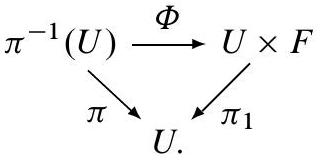
\includegraphics[max width=\textwidth, center]{2025_06_03_90f64b1a1e243cccc2e0g-286}

The space $E$ is called the total space of the bundle, $M$ is its base, and $\pi$ is its projection. If $E, M$, and $F$ are smooth manifolds with or without boundary, $\pi$ is a smooth map, and the local trivializations can be chosen to be diffeomorphisms, then it is called a smooth fiber bundle.

A trivial fiber bundle is one that admits a local trivialization over the entire base space (a global trivialization). It is said to be smoothly trivial if it is a smooth bundle and the global trivialization is a diffeomorphism.

\section*{Example 10.37 (Fiber Bundles).}
(a) Every product space $M \times F$ is a fiber bundle with projection $\pi_{1}: M \times F \rightarrow M$, called a product fiber bundle. It has a global trivialization given by the identity map $M \times F \rightarrow M \times F$, so every product bundle is trivial.\\
(b) Every rank- $k$ vector bundle is a fiber bundle with model fiber $\mathbb{R}^{k}$.\\
(c) If $E \rightarrow \mathbb{S}^{1}$ is the Möbius bundle of Example 10.3, then the image of $\mathbb{R} \times[-1,1]$ under the quotient map $q: \mathbb{R}^{2} \rightarrow E$ is a fiber bundle over $\mathbb{S}^{1}$ with model fiber $[-1,1]$. It is not a trivial bundle. (Can you prove it?)\\
(d) Every covering map $\pi: E \rightarrow M$ is a fiber bundle whose model fiber is discrete. To construct local trivializations, let $S$ be a discrete space with the same cardinality as the fibers of $\pi$. For each evenly covered open subset $U \subseteq M$, define a map $\Phi: \pi^{-1}(U) \rightarrow U \times S$ by choosing a bijection between the set of components of $\pi^{-1}(U)$ and $S$, and letting $\Phi(x)=(\pi(x), c(x))$, where $c(x)$ is the element of $S$ corresponding to the component containing $x$. //

We will see a few more examples of fiber bundles as we go along.

\section*{Problems}
10-1. Let $E$ be the total space of the Möbius bundle constructed in Example 10.3.\\
(a) Show that $E$ has a unique smooth structure such that the quotient map $q: \mathbb{R}^{2} \rightarrow E$ is a smooth covering map.\\
(b) Show that $\pi: E \rightarrow \mathbb{S}^{1}$ is a smooth rank-1 vector bundle.\\
(c) Show that it is not a trivial bundle.

10-2. Let $E$ be a vector bundle over a topological space $M$. Show that the projection map $\pi: E \rightarrow M$ is a homotopy equivalence.\\
10-3. Let VB denote the category whose objects are smooth vector bundles and whose morphisms are smooth bundle homomorphism, and let Diff denote the category whose objects are smooth manifolds and whose morphisms are smooth maps. Show that the assignment $M \mapsto T M, F \mapsto d F$ defines a covariant functor from Diff to VB, called the tangent functor. (Used on p. 303.)\\
10-4. Complete the proof of Lemma 10.5 by showing that $\tau: U \cap V \rightarrow \mathrm{GL}(k, \mathbb{R})$ is smooth. [Hint: use the same idea as in the proof of Proposition 7.37.]\\
10-5. Let $\pi: E \rightarrow M$ be a smooth vector bundle of rank $k$ over a smooth manifold $M$ with or without boundary. Suppose that $\left\{U_{\alpha}\right\}_{\alpha \in A}$ is an open cover of $M$, and for each $\alpha \in A$ we are given a smooth local trivialization $\Phi_{\alpha}: \pi^{-1}\left(U_{\alpha}\right) \rightarrow U_{\alpha} \times \mathbb{R}^{k}$ of $E$. For each $\alpha, \beta \in A$ such that $U_{\alpha} \cap U_{\beta} \neq \varnothing$, let $\tau_{\alpha \beta}: U_{\alpha} \cap U_{\beta} \rightarrow \mathrm{GL}(k, \mathbb{R})$ be the transition function defined by (10.3). Show that the following identity is satisfied for all $\alpha, \beta, \gamma \in A$ :

$$
\tau_{\alpha \beta}(p) \tau_{\beta \gamma}(p)=\tau_{\alpha \gamma}(p), \quad p \in U_{\alpha} \cap U_{\beta} \cap U_{\gamma}
$$

(The juxtaposition on the left-hand side represents matrix multiplication.)\\
10-6. Vector Bundle Construction Theorem: Let $M$ be a smooth manifold with or without boundary, and let $\left\{U_{\alpha}\right\}_{\alpha \in A}$ be an open cover of $M$. Suppose for each $\alpha, \beta \in A$ we are given a smooth map $\tau_{\alpha \beta}: U_{\alpha} \cap U_{\beta} \rightarrow$ $\mathrm{GL}(k, \mathbb{R})$ such that (10.7) is satisfied for all $\alpha, \beta, \gamma \in A$. Show that there is a smooth rank- $k$ vector bundle $E \rightarrow M$ with smooth local trivializations $\Phi_{\alpha}: \pi^{-1}\left(U_{\alpha}\right) \rightarrow U_{\alpha} \times \mathbb{R}^{k}$ whose transition functions are the given maps $\tau_{\alpha \beta}$. [Hint: define an appropriate equivalence relation on $\bigsqcup_{\alpha \in A}\left(U_{\alpha} \times \mathbb{R}^{k}\right)$, and use the vector bundle chart lemma.]\\
10-7. Compute the transition function for $T \mathbb{S}^{2}$ associated with the two local trivializations determined by stereographic coordinates (Problem 1-7).\\
10-8. Let $\mathrm{Vec}_{1}$ be the category whose objects are finite-dimensional real vector spaces and whose morphisms are linear isomorphisms. If $\mathscr{F}$ is a covariant functor from $\mathrm{Vec}_{1}$ to itself, for each finite-dimensional vector space $V$ we get a map $\mathscr{F}: \operatorname{GL}(V) \rightarrow \operatorname{GL}(\mathscr{F}(V))$ sending each isomorphism $A: V \rightarrow V$ to the induced isomorphism $\mathscr{F}(A): \mathscr{F}(V) \rightarrow \mathscr{F}(V)$. We say $\mathscr{F}$ is a smooth functor if this map is smooth for every $V$. Given a smooth vector bundle $E \rightarrow M$ and a smooth functor $\mathcal{F}: \operatorname{Vec}_{1} \rightarrow \operatorname{Vec}_{1}$, show that there is a smooth vector bundle $\mathscr{F}(E) \rightarrow M$ whose fiber at each point $p \in M$ is $\mathcal{F}\left(E_{p}\right)$. (Used on p. 299.)


\end{document}